% -*- coding: utf-8 -*-

\chapter{绪论}

\section{研究背景与问题挑战}

指数增强（Index Enhancement）策略介于完全被动的指数跟踪与完全主动的证券选择之间，其目标是在严格控制相对基准跟踪误差的前提下，系统性地获取稳定的超额收益，即所谓 ``Beta 稳健、Alpha 突出''。本文以中国 A 股市场的核心宽基基准——\textbf{沪深 300 指数}为实证标的，研究指数增强策略中核心量化算法的优化设计与实现。

从计算的视角看，一个完整的指数增强策略可抽象为两个串联环节：其一是\emph{信号生成}，即由多源因子预测个股的截面超额收益（alpha）；其二是\emph{组合构建}，即在给定 alpha 预测的条件下，求解一组满足风险与交易约束的可实施权重。前者本质上是一个有监督的截面回归问题，后者则是一个带约束的数学规划问题。本文研究的核心，正是第二个环节——\textbf{带约束的组合优化算法}，因为它直接决定了预测信号能在多大程度上、以多稳健的方式转化为真实可交易的主动头寸。

组合优化在指数增强中的核心地位，可由主动管理基本定律精确刻画。Grinold\cite{Grinold1989} 将信息比率（$IR$）分解为预测能力（$IC$）与投资广度（$N$）的乘积 $IR = IC\cdot\sqrt{N}$；Clarke 等\cite{Clarke2002} 进一步引入传输系数（Transfer Coefficient，$TC$），将其修正为
\[
IR = TC\cdot IC\cdot\sqrt{N},\qquad TC\in[0,1].
\]
其中 $TC$ 度量了组合优化器将理论 alpha 信号 ``传输'' 为实际主动权重的效率。禁止卖空、行业中性、跟踪误差上限与换手率上限等现实约束会系统性地压低 $TC$\cite{Grinold2000,Ding2017}。因此，\emph{在严苛的多面体约束空间内构造一个使 $TC$ 最大化、且数值稳健的优化算法}，构成了指数增强策略落地的核心难题。

在 A 股市场，这一难题面临两重叠加的挑战。

\textbf{挑战一：协方差病态与 ``误差最大化''。}组合优化的风险项依赖于个股收益协方差矩阵的估计。当资产数（沪深 300 约 300 只）与估计窗口长度相当时，样本协方差矩阵呈病态，其最小特征值接近零甚至为负。Michaud\cite{Michaud1989} 指出，直接使用此类矩阵的均值-方差优化器会放大估计误差，倾向于在被高估的资产上给出极端权重，即 ``误差最大化''（Error Maximization）。如何在估计层面抑制病态、在求解层面保证数值稳健，是优化算法必须解决的工程问题。

\textbf{挑战二：低信噪比下的预测不确定性。}A 股以散户交易为主、错误定价频繁、风格切换剧烈，截面 alpha 预测的信噪比极低且高度非平稳。传统组合优化器只接收 alpha 的\emph{点预测}，默认所有个股的预测同等可信，完全忽略了不同个股之间预测可信度的差异。在低信噪比环境下，这种 ``一视同仁'' 会让优化器把大量权重押注在高方差、低可信度的预测上。因此，如何为 alpha 预测附加一个有理论保证的不确定性度量，并将其纳入优化算法，是提升策略稳健性的关键。

\section{主要工作与论文结构}
\label{sec:contributions}

针对上述挑战，本文围绕指数增强的核心组合优化算法展开优化设计与实现，主要工作包括两个层面。

\textbf{（一）面向 A 股的约束型多因子组合优化算法。}本文以 LightGBM\cite{Ke2017LightGBM} 多因子模型输出截面 alpha 信号，针对挑战一，采用 Ledoit-Wolf 缩减估计\cite{Ledoit2004} 抑制样本协方差病态，并在求解层附加最小特征值修正以保证半正定；在此基础上构建以 alpha 收益、风险惩罚与换手惩罚为目标、以跟踪误差、行业偏离、单股权重与换手率为约束的二次规划（QP），并设计 OSQP$\to$CLARABEL$\to$SCS 三级求解器回退机制保证数值鲁棒性。该算法将信息比率由静态多因子的 0.237 提升至 2.449。

\textbf{（二）不确定性感知的组合优化扩展。}针对挑战二，本文将 Split 与 Mondrian Conformal Prediction\cite{Vovk2005Conformal,Romano2019CQR,Angelopoulos2021Gentle} 引入组合优化：为每只股票的 alpha 预测构造具有有限样本边际覆盖保证的预测区间，并由区间半宽导出归一化置信度 $c_i$；进而设计 alpha 缩放、候选过滤与目标惩罚三种置信加权方案，将 $c_i$ 分别耦合进 QP 的目标项与可行域。本文对该扩展在 A 股的行为进行了系统评估，揭示出名义 $90\%$ 区间存在约 $9$ 个百分点的系统性低覆盖（且与显著性水平无关）与 ``高置信即过拟合'' 的反向规律，并通过简化的自适应 Conformal 推断模拟给出了矫正约 $80\%$ 覆盖偏差的可行路径。

本文使用的主要数学符号汇总于表~\ref{tab:symbols}。

\begin{table}[htbp]
\centering
\caption{主要数学符号}
\label{tab:symbols}
\begin{tabular}{ll}
\toprule
\textbf{符号} & \textbf{含义} \\
\midrule
$IR,\ IC,\ N,\ TC$ & 信息比率、因子信息系数、投资广度、传输系数 \\
$w\in\mathbb{R}^n$ & 组合权重向量；$w_b$ 为基准权重，$w_{\text{prev}}$ 为上期权重 \\
$\hat\alpha\in\mathbb{R}^n$ & 标准化后的截面 alpha 预测分数向量 \\
$\Sigma\in\mathbb{R}^{n\times n}$ & 个股日收益协方差矩阵（Ledoit-Wolf 缩减估计） \\
$\lambda,\ \kappa$ & 风险厌恶系数、换手惩罚系数 \\
$\sigma_{TE}$ & 年化跟踪误差上限 \\
$\alpha_{\text{CP}},\ q_{\alpha}$ & Conformal 显著性水平、校准残差分位数（区间半宽） \\
$c_i$ & 第 $i$ 只股票的归一化 Conformal 置信度 \\
$\beta,\ \gamma,\ p_{\text{top}}$ & 三种置信加权方案的参数 \\
$\rho$ & 校准集占训练样本的比例 \\
$n_d,\ n_s$ & 回测面板的交易日数与股票数 \\
\bottomrule
\end{tabular}
\end{table}

全文共五章。第一章为绪论，交代研究背景，明确以约束组合优化为核心的研究问题及其在 A 股的两重挑战，并概述主要工作。第二章为背景知识与相关工作，分别梳理指数增强与组合优化的理论基础、以及不确定性量化与 Conformal Prediction 的相关进展。第三章为核心章，先给出系统整体框架与架构图，再依次详述约束型多因子组合优化算法及其不确定性感知扩展的设计与实现，并以伪代码严格表达算法逻辑、给出复杂度分析。第四章为实验与分析，在长周期（2015--2024）与短周期（2024--2025）两条样本上，通过与基线的对比论证算法的有效性，并对不确定性感知扩展的行为给出深入分析。第五章总结全文工作并讨论局限与未来方向。

\chapter{背景知识与相关工作}

\section{指数增强与组合优化的理论基础}

\subsection{主动管理基本定律与传输系数}
量化主动管理的数学基础由 Grinold\cite{Grinold1989} 奠定，其将信息比率分解为预测能力与投资广度的乘积 $IR=IC\cdot\sqrt{N}$。该原始定律隐含 ``所有 alpha 信号均可无摩擦地转化为主动头寸'' 的理想假设。Ding 与 Martin\cite{Ding2017} 指出，由于资产残差相关与横截面信息非平稳，盲目套用原始定律会显著高估实盘 $IR$。Clarke 等\cite{Clarke2002} 引入传输系数 $TC$，将定律修正为 $IR=TC\cdot IC\cdot\sqrt{N}$，并证明禁止卖空与各类风险约束会使 $TC$ 远小于 1；Grinold 与 Kahn\cite{Grinold2000} 的经典教材进一步将其系统化为现代主动管理的方法学基础。这一理论框架表明，指数增强策略的绩效上限由信号质量（$IC$）决定，而其实际兑现程度由组合优化器的传输效率（$TC$）决定，从而确立了组合优化在策略中的核心地位。

\subsection{均值-方差优化与协方差缩减}
Markowitz 框架下的均值-方差组合优化以二次规划形式求解收益与风险的权衡。然而其对输入参数高度敏感：Michaud\cite{Michaud1989} 指出，由历史收益直接估计的样本协方差矩阵在高维下呈病态，会诱导优化器产生集中于估计误差方向的极端 ``角点解''，即 ``误差最大化''。Ledoit 与 Wolf\cite{Ledoit2004} 提出线性收缩估计，将高方差的样本协方差矩阵按最优强度向结构化目标矩阵收缩，可显著平滑极端系数、降低实现跟踪误差，是组合优化中协方差估计的标准做法。本文的优化算法在协方差估计层采用 Ledoit-Wolf 缩减，并在求解层附加最小特征值修正，二者共同应对挑战一。

\subsection{因子模型与机器学习在 A 股的实证}
Fama 与 French\cite{Fama2015} 的五因子模型在成熟市场具有较强解释力，但在 A 股，受宏观调控与散户结构影响，投资因子常常冗余，而流动性与动量溢价更为显著，直接套用西方框架易失效。Gu 等\cite{Gu2020} 的开创性工作确立了机器学习在实证资产定价中的基准，证明非线性树模型与神经网络能够捕获因子间的条件触发与高阶交互，预测精度全面超越线性回归。Chen 等\cite{Chen2024DeepLearningAP} 进一步证实，结合宏观状态变量与非线性模型可显著改善 A 股截面预测。Yang\cite{Yang2025} 则验证了 LightGBM 在低信噪比 A 股环境下的工程优势。基于上述结论，本文以 LightGBM 多因子模型作为组合优化算法的上游 alpha 信号来源。

\section{不确定性量化与 Conformal Prediction}

\subsection{Conformal Prediction 的理论保证}
Conformal Prediction（CP）由 Vovk 等\cite{Vovk2005Conformal} 提出，其在仅假设数据可交换性（exchangeability）的弱条件下，即可为任意点预测构造具有\emph{有限样本边际覆盖保证}的预测区间。Split Conformal 通过将训练集划分为建模子集与校准子集，以校准残差的经验分位数作为区间半宽，计算高效且与底层模型解耦。Romano 等\cite{Romano2019CQR} 的 Conformalized Quantile Regression 借助分位数回归改善条件覆盖，在异方差场景下优于经典 Split CP。Angelopoulos 与 Bates\cite{Angelopoulos2021Gentle} 系统梳理了 CP 的实践范式。Mondrian Conformal 则按离散组别（如行业）独立校准，以缓解组间预测难度不均导致的覆盖偏差。本文以 Split 与 Mondrian CP 为 alpha 预测附加置信度，应对挑战二。

\subsection{金融场景下的覆盖偏差与自适应改进}
CP 的边际覆盖保证依赖可交换性，而金融时序的截面相关与时间漂移会破坏该假设，使实测覆盖偏离名义水平。Kato\cite{Kato2024CPPS} 将 CP 直接嵌入组合选择，提出 Conformal Predictive Portfolio Selection 范式，与本文的不确定性感知优化高度相关。为应对分布漂移，Gibbs 与 Cand\`es\cite{Gibbs2021ACI} 提出 Adaptive Conformal Inference（ACI），通过在线调整名义 miscoverage 率使长期覆盖收敛；Xu 与 Xie\cite{Xu2023SPCI} 引入残差自相关建模改善时序覆盖；Aydin 等\cite{Aydin2025TCP} 的 Temporal Conformal Prediction、Yang 等\cite{Yang2025ECI} 的 Error-quantified Conformal Inference、Sun 等\cite{Sun2025CPTC} 的变点感知 CP 以及 Neglia 等\cite{Neglia2026ResCP} 的免训练 ResCP，进一步提升了覆盖自适应性。本文在实验中以简化的 ACI 模拟验证了这一改进路径在 A 股环境下矫正覆盖偏差的潜力（第~\ref{sec:future_work} 节）。

\section{本章小结}
本章梳理了与本文核心算法相关的两类理论与工作：其一是指数增强与组合优化的理论基础，主动管理基本定律确立了组合优化（最大化 $TC$）在策略中的核心地位，协方差缩减则为应对病态提供了方法；其二是不确定性量化与 Conformal Prediction，为在低信噪比环境下量化 alpha 预测可信度提供了具有理论保证的工具。这些工作共同构成了第三章算法设计的出发点。

\chapter{指数增强组合优化算法的设计与实现}

本章是全文的核心。第~\ref{sec:framework} 节给出系统整体框架，明确核心算法在系统中的位置；第~\ref{sec:cpo} 节详述约束型多因子组合优化算法的设计、伪代码与复杂度；第~\ref{sec:uaco} 节给出其不确定性感知扩展。

\section{系统整体框架}
\label{sec:framework}

本文的指数增强系统由六个层次串联而成，整体架构如图~\ref{fig:arch} 所示。数据层经由 \texttt{akshare} 与 \texttt{baostock} 接入沪深 300 成分股的行情、季度财务与宏观数据；因子工程层将其加工为 15 个数值因子并完成异常值控制与截面标准化；alpha 预测层由 LightGBM 多因子模型输出截面 alpha 分数 $\hat\alpha$；不确定性量化层以 Conformal Prediction 为每只股票的预测附加置信度 $c_i$；组合优化层求解带约束的二次规划，输出主动权重 $w$；回测评估层以月度调仓并计入双边交易成本，输出 $IR$、Sharpe、最大回撤等绩效指标。

\begin{figure}[htbp]
\centering
\begin{tikzpicture}[
  box/.style={draw, rounded corners, align=center, text width=10.2cm, minimum height=0.82cm, font=\small},
  core/.style={draw, rounded corners, align=center, text width=10.2cm, minimum height=0.82cm, font=\small, fill=black!6},
  arr/.style={-{Latex[length=2.2mm]}, thick},
  node distance=0.5cm,
]
\node[box] (data) {数据层：\texttt{akshare} / \texttt{baostock} 行情、季度财务、宏观（北向、M2、利差）};
\node[box, below=of data] (factor) {因子工程层：15 个因子 $\cdot$ MAD 缩尾 $\cdot$ 截面 Z-Score $\cdot$ 行业中性化};
\node[box, below=of factor] (alpha) {Alpha 预测层：LightGBM 多因子模型 $\Rightarrow$ 截面 alpha 分数 $\hat\alpha$};
\node[core, below=of alpha] (cp) {不确定性量化层：Split / Mondrian Conformal Prediction $\Rightarrow$ 置信度 $c_i$};
\node[core, below=of cp] (opt) {组合优化层：约束二次规划（Ledoit-Wolf 协方差 $+$ 多面体约束 $+$ 置信加权）$\Rightarrow$ 权重 $w$};
\node[box, below=of opt] (bt) {回测评估层：月度调仓 $+$ 双边交易成本 $\Rightarrow$ $IR$ / Sharpe / 最大回撤};
\draw[arr] (data)--(factor);
\draw[arr] (factor)--(alpha);
\draw[arr] (alpha)--(cp);
\draw[arr] (cp)--(opt);
\draw[arr] (opt)--(bt);
\begin{scope}[on background layer]
\node[draw, dashed, rounded corners, fit=(cp)(opt), inner sep=0.22cm] (corebox) {};
\end{scope}
\end{tikzpicture}
\caption{指数增强系统整体架构（虚线框为本文核心算法）}
\label{fig:arch}
\end{figure}

在该框架中，本文的核心算法位于图~\ref{fig:arch} 的虚线框内，即不确定性量化层与组合优化层。alpha 预测层提供输入信号，回测评估层提供输出度量，二者为核心算法的设计与评估提供了完整的上下文。值得强调的是，alpha 预测层与组合优化层是\emph{解耦}的：优化算法只接收标准化的 alpha 分数与（可选的）置信度，而不依赖具体的预测模型，这使得算法可独立替换上游模型、便于消融与复用。

为完整起见，本节先简述上游因子工程与 alpha 预测的设定。本文使用 15 个数值因子，按语义分为四组：价值（\texttt{ep\_ttm}、\texttt{bp}）、质量（\texttt{roe}、\texttt{grossprofitmargin}、\texttt{netprofitmargin}、\texttt{yoynetprofit}、\texttt{assetturnover}、\texttt{cfotoor}）、技术与微观结构（\texttt{ret\_20}、\texttt{ret\_60}、\texttt{volatility\_20}、\texttt{turnover\_20}）、外部宏观（\texttt{northbound\_net\_inflow}、\texttt{m2\_yoy}、\texttt{cn\_spread\_10y\_2y}）。每个因子在每个交易日截面上依次经过 MAD 缩尾（$k=3$）、Z-Score 标准化与行业中性化处理。预测标签采用相对沪深 300 的 20 日超额收益，以剥离系统性 Beta、聚焦截面 alpha。alpha 预测层采用固定超参数的 LightGBM（\texttt{n\_estimators=300}、\texttt{learning\_rate=0.05}、\texttt{num\_leaves=31}），以月度滚动方式重训。

\section{约束型多因子组合优化算法}
\label{sec:cpo}

\subsection{优化问题的形式化}
设某调仓日截面含 $n$ 只股票，记 $\hat\alpha\in\mathbb{R}^n$ 为标准化 alpha 分数，$w\in\mathbb{R}^n$ 为待求组合权重，$w_b$ 为基准权重，$w_{\text{prev}}$ 为上期权重，$\Sigma\in\mathbb{R}^{n\times n}$ 为个股日收益协方差矩阵，主动权重为 $w-w_b$。本文将组合优化形式化为如下二次规划：
\begin{align}
\max_{w}\quad & \hat\alpha^\top w \;-\; \lambda\,(w-w_b)^\top \Sigma\,(w-w_b)\;-\;\kappa\,\lVert w-w_{\text{prev}}\rVert_1 \label{eq:obj}\\
\text{s.t.}\quad & \mathbf{1}^\top w = 1,\qquad 0 \le w_i \le w_{\max}, \label{eq:box}\\
& (w-w_b)^\top \Sigma\,(w-w_b) \;\le\; \big(\sigma_{TE}/\sqrt{252}\big)^2, \label{eq:te}\\
& \big|\,\mathbf{1}_{S_k}^\top (w-w_b)\,\big| \;\le\; d_{\text{ind}},\quad \forall\,k, \label{eq:ind}\\
& \lVert w-w_{\text{prev}}\rVert_1 \;\le\; 2\,\tau_{\max}. \label{eq:turn}
\end{align}
目标式~\eqref{eq:obj} 由三项构成：alpha 收益项 $\hat\alpha^\top w$、以风险厌恶系数 $\lambda$ 加权的主动风险惩罚项、以及以 $\kappa$ 加权的 $\ell_1$ 换手惩罚项。约束式~\eqref{eq:box} 为全额投资与禁止卖空、单股权重上限 $w_{\max}$；式~\eqref{eq:te} 将\emph{事前年化跟踪误差}约束在 $\sigma_{TE}$ 以内（其中 $\Sigma$ 为日频协方差，$\sqrt{252}$ 为年化因子）；式~\eqref{eq:ind} 限制每个申万一级行业 $S_k$ 的主动暴露不超过 $d_{\text{ind}}$；式~\eqref{eq:turn} 将月度单边换手约束在 $\tau_{\max}$ 以内。该问题是一个带二次约束的凸二次规划，全局最优解存在且唯一（当 $\Sigma$ 半正定时）。约束式~\eqref{eq:te}--\eqref{eq:turn} 正是压低传输系数 $TC$、却保证策略可实施性的现实摩擦，优化算法的任务即在该可行域内最大化 alpha 兑现。

\subsection{协方差估计与数值稳健性}
协方差矩阵 $\Sigma$ 的质量直接决定式~\eqref{eq:obj} 与式~\eqref{eq:te} 的可靠性。本文采用 Ledoit-Wolf 缩减估计\cite{Ledoit2004}：取调仓日前 $60$ 个交易日的个股日收益，缺失以 $0$ 填充后，按最优收缩强度将样本协方差向缩减目标加权，得到良态估计 $\hat\Sigma_{\text{LW}}$。为进一步保证求解器所需的半正定性，本文对 $\hat\Sigma_{\text{LW}}$ 做对称化并计算最小特征值 $\mu_{\min}$：若 $\mu_{\min}<0$，则加上 $(-\mu_{\min}+\epsilon)I$ 修正；否则加上 $\epsilon I$ 的 ridge 项（$\epsilon=10^{-4}$）。该 ``缩减 $+$ 特征值修正'' 的两级处理共同抑制了挑战一中的 ``误差最大化''。

在求解层面，本文设计了 OSQP$\to$CLARABEL$\to$SCS 的三级求解器回退机制：优先以高精度参数调用一阶算子分裂法 OSQP，若其未能返回最优解，则依次降级到内点法 CLARABEL 与一阶锥求解器 SCS；若三者均失败，则回退到上期权重 $w_{\text{prev}}$（或基准权重）以保证回测链路不中断。求解结果再经裁剪与归一化以严格满足式~\eqref{eq:box}。该机制以可控的额外开销换取了长周期回测中数千次连续求解的鲁棒性。

\subsection{算法描述与复杂度}
约束型多因子组合优化的完整流程如算法~\ref{alg:cpo} 所示。

\begin{algorithm}[htbp]
\caption{约束型多因子组合优化（单期调仓）}
\label{alg:cpo}
\begin{algorithmic}[1]
\Require 截面快照（含 $\hat\alpha$、$w_b$、行业标签）、历史日收益 $R$、上期权重 $w_{\text{prev}}$、配置 $(\lambda,\kappa,\sigma_{TE},d_{\text{ind}},w_{\max},\tau_{\max})$
\Ensure 主动权重 $w$ 与诊断量（事前跟踪误差、换手、最大行业偏离）
\State 清洗截面，删除缺失 $\hat\alpha$ 的样本；归一化 $w_b$ 使 $\mathbf{1}^\top w_b=1$
\State 对 $\hat\alpha$ 做截面去均值除标准差，得标准化分数
\State $\hat\Sigma_{\text{LW}} \gets \textsc{LedoitWolf}(R\text{ 的近 }60\text{ 日截面})$ \Comment{协方差缩减}
\State 对称化 $\hat\Sigma_{\text{LW}}$；计算 $\mu_{\min}$；按符号施加特征值修正或 ridge 项，得 $\Sigma$
\State 构造行业指示矩阵 $\{\mathbf{1}_{S_k}\}$ 与基准行业暴露
\State 按式~\eqref{eq:obj}--\eqref{eq:turn} 组装目标与约束
\For{$\textit{solver} \in \{\text{OSQP},\text{CLARABEL},\text{SCS}\}$}
  \State 以 $\textit{solver}$ 求解 QP
  \If{状态为最优且解非空}
    \State 裁剪到 $[0,w_{\max}]$ 并归一化；\textbf{return} $w$ 与诊断量
  \EndIf
\EndFor
\State \textbf{return} 回退权重 $w_{\text{prev}}$（或 $w_b$）
\end{algorithmic}
\end{algorithm}

\textbf{复杂度分析。}设单期截面股票数为 $n$、协方差估计窗口为 $T$（本文 $T=60$）。协方差缩减估计的代价为 $O(n^2 T)$，最小特征值计算为 $O(n^3)$。二次规划含 $n$ 个变量、$O(n+m)$ 个约束（$m$ 为行业数），一阶或内点求解器单次迭代的主导代价为 $O(n^3)$。因此单期调仓的时间复杂度为 $O(n^3 + n^2 T)$，空间复杂度为 $O(n^2)$。对一个含 $n_d$ 个交易日、月度调仓共 $R$ 次的回测，总复杂度为 $O\big(R\,(n^3+n^2 T)\big)$。在 $n\approx 300$、$R\approx 120$ 的长周期设定下，该复杂度可在单机 CPU 上分钟级完成，无需 GPU 依赖。

\section{不确定性感知的组合优化扩展}
\label{sec:uaco}

\subsection{基于 Conformal Prediction 的置信度构造}
为应对挑战二，本文在 alpha 预测之上引入 Split Conformal Prediction，为每只股票构造置信度。对每个滚动训练窗口，将训练子集按 $1-\rho:\rho$（$\rho=0.3$）随机划分为建模子集 $D_{\text{tr}}$ 与校准子集 $D_{\text{cal}}$；底层模型在 $D_{\text{tr}}$ 上拟合后，在 $D_{\text{cal}}$ 上计算保形得分 $s_i=|y_i-\hat y_i|$，并取其 Vovk 修正分位数
\[
q_\alpha = \text{Quantile}_{\,\lceil (n_{\text{cal}}+1)(1-\alpha_{\text{CP}})\rceil/n_{\text{cal}}}\big(\{s_i\}\big),
\]
其中 $\alpha_{\text{CP}}=0.1$ 对应名义 $90\%$ 覆盖。测试样本的预测区间为 $[\hat y - q_\alpha,\ \hat y + q_\alpha]$，半宽越小表示预测越可信。据此定义原始置信度 $\tilde c_i = 1/(2q_{\alpha,i}+\epsilon)$，再经 min-max 归一化得 $c_i\in[0,1]$。Mondrian 变体按申万一级行业分组独立计算 $q_\alpha$（组样本不足时回退全局分位数），以实现条件覆盖。该过程如算法~\ref{alg:cp} 所示。

\begin{algorithm}[htbp]
\caption{Split Conformal 校准与置信度构造}
\label{alg:cp}
\begin{algorithmic}[1]
\Require 训练特征 $X$、标签 $y$、模型工厂、校准比例 $\rho$、显著性水平 $\alpha_{\text{CP}}$
\Ensure 各测试样本的置信度 $\{c_i\}$
\State 将 $(X,y)$ 随机划分为建模子集 $D_{\text{tr}}$ 与校准子集 $D_{\text{cal}}$（比例 $1-\rho:\rho$）
\State 在 $D_{\text{tr}}$ 上拟合底层模型，得 $\hat f$
\State 在 $D_{\text{cal}}$ 上计算保形得分 $s_i=|y_i-\hat f(x_i)|$
\State $q_\alpha \gets$ $\{s_i\}$ 的 Vovk 修正 $(1-\alpha_{\text{CP}})$ 分位数
\State 对测试样本，半宽 $\gets q_\alpha$（Mondrian 取所在行业的 $q_\alpha$）
\State $\tilde c_i \gets 1/(2\cdot\text{半宽}_i+\epsilon)$；min-max 归一化得 $c_i$
\State \textbf{return} $\{c_i\}$
\end{algorithmic}
\end{algorithm}

\subsection{三种置信加权方案}
本文设计三种方案，将置信度 $c_i$ 耦合进算法~\ref{alg:cpo} 的优化问题，以体现 ``可信度高的预测获得更大权重自由度'' 这一直觉：
\begin{itemize}
    \item \textbf{alpha 缩放}（\texttt{alpha\_scale}）：在目标项中以 $\hat\alpha_i' = \hat\alpha_i\cdot c_i^{\beta}$ 替换原 alpha（$\beta=1$ 默认），直接放大高置信样本的收益贡献；
    \item \textbf{候选过滤}（\texttt{candidate\_filter}）：仅保留置信度排名前 $p_{\text{top}}$（$=70\%$）的股票进入 QP 候选池（至少保留 $30$ 只），其余权重置零，从可行域层面剔除低可信样本；
    \item \textbf{目标惩罚}（\texttt{objective\_penalty}）：在目标式~\eqref{eq:obj} 中追加惩罚项 $-\gamma\sum_i (1-c_i)\,w_i^2$（$\gamma=0.1$ 默认），对低置信样本的权重施加二次抑制。
\end{itemize}
三种方案分别从\emph{目标系数、可行域、目标曲率}三个不同层面注入不确定性信息，构成一个由温和到激进的谱系：目标惩罚最温和（仅二次抑制），候选过滤居中（硬性剔除），alpha 缩放最激进（直接重标定收益）。整体流程如图~\ref{fig:ua_flow} 所示。当截面缺少置信度列时，扩展算法自动退化为算法~\ref{alg:cpo}，保证向后兼容。

\begin{figure}[htbp]
\centering
\resizebox{\textwidth}{!}{%
\begin{tikzpicture}[
  b/.style={draw, rounded corners, align=center, font=\small, minimum height=0.8cm, inner sep=3pt},
  arr/.style={-{Latex[length=2mm]}, thick},
  node distance=0.55cm and 0.9cm,
]
\node[b, text width=2.4cm] (cal) {Conformal 校准\\$q_\alpha$（算法~\ref{alg:cp}）};
\node[b, right=of cal, text width=2.2cm] (conf) {置信度 $c_i$\\$=1/(2q_\alpha{+}\epsilon)$};
\node[b, right=of conf, text width=2.0cm] (as) {\texttt{alpha\_scale}\\$\hat\alpha_i c_i^{\beta}$};
\node[b, below=of as, text width=2.0cm] (cf) {\texttt{candidate\_filter}\\保留 top $p_{\text{top}}$};
\node[b, above=of as, text width=2.0cm] (op) {\texttt{objective\_penalty}\\$-\gamma(1{-}c_i)w_i^2$};
\node[b, right=2.0cm of as, text width=2.0cm] (qp) {约束 QP\\（算法~\ref{alg:cpo}）};
\node[b, right=of qp, text width=1.4cm] (w) {权重 $w$};
\draw[arr] (cal)--(conf);
\draw[arr] (conf)--(as);
\draw[arr] (conf.east) to[out=-20,in=180] (cf.west);
\draw[arr] (conf.east) to[out=20,in=180] (op.west);
\draw[arr] (as)--(qp);
\draw[arr] (op.east) to[out=0,in=160] (qp.north west);
\draw[arr] (cf.east) to[out=0,in=200] (qp.south west);
\draw[arr] (qp)--(w);
\end{tikzpicture}%
}
\caption{不确定性感知组合优化流程：置信度经三种方案之一耦合进约束 QP}
\label{fig:ua_flow}
\end{figure}

\subsection{不确定性感知优化算法}
不确定性感知组合优化的完整流程如算法~\ref{alg:uaco} 所示。它在算法~\ref{alg:cpo} 的基础上，依据所选方案在 ``信号注入''（alpha 缩放）、``候选筛选''（候选过滤）或 ``目标改写''（目标惩罚）三处之一插入置信度，其余协方差估计、约束组装与求解器回退逻辑完全复用，体现了与基础算法的正交解耦。

\begin{algorithm}[htbp]
\caption{不确定性感知组合优化（单期调仓）}
\label{alg:uaco}
\begin{algorithmic}[1]
\Require 截面快照（含 $\hat\alpha$、$w_b$、置信度 $c$）、历史日收益 $R$、$w_{\text{prev}}$、方案 $\in\{\texttt{alpha\_scale},\texttt{candidate\_filter},\texttt{objective\_penalty}\}$ 及其参数 $(\beta,p_{\text{top}},\gamma)$
\Ensure 主动权重 $w$
\If{截面无置信度列}
  \State \textbf{return} 算法~\ref{alg:cpo} 的结果 \Comment{向后兼容}
\EndIf
\State 将 $c$ 截断到 $[0,1]$，缺失以中位数填充
\If{方案 $=\texttt{candidate\_filter}$}
  \State 按 $c$ 降序保留前 $\lceil p_{\text{top}}\, n\rceil$ 只（至少 $30$ 只）
\EndIf
\State 执行算法~\ref{alg:cpo} 的步骤 1--5（清洗、标准化、协方差、行业矩阵）
\If{方案 $=\texttt{alpha\_scale}$}
  \State $\hat\alpha \gets \hat\alpha \odot c^{\beta}$ \Comment{逐元素缩放}
\EndIf
\If{方案 $=\texttt{objective\_penalty}$}
  \State 在目标中追加 $-\gamma\sum_i (1-c_i)\,w_i^2$
\EndIf
\State 经三级求解器回退求解 QP；裁剪并归一化
\State \textbf{return} $w$
\end{algorithmic}
\end{algorithm}

至此，本文完成了对指数增强核心组合优化算法的设计与实现：算法~\ref{alg:cpo} 以协方差缩减、特征值修正与求解器回退应对挑战一，算法~\ref{alg:cp}--\ref{alg:uaco} 以 Conformal 置信度的三种耦合方式应对挑战二。下一章将在真实 A 股数据上对二者进行系统的实验评估。

\chapter{实验与分析}

本章在沪深 300 真实数据上评估第三章算法。第~\ref{sec:exp_setup} 节交代实验环境、数据集与方案；第~\ref{sec:exp_results} 节给出结果并展开深入分析与对比论证；第~\ref{sec:exp_summary} 节小结。

\section{实验环境与方案}
\label{sec:exp_setup}

\subsection{软硬件环境与数据集}
全部实验在 Apple Silicon M 系列 CPU 单机完成，软件环境为 Python 3.11，组合优化由 \texttt{cvxpy} 调用 OSQP/CLARABEL/SCS 求解，alpha 模型为 \texttt{lightgbm}，协方差缩减与 Conformal 校准依赖 \texttt{scikit-learn}。全流程 CPU 友好、无 GPU 依赖。

实验使用两条样本。\textbf{长周期样本}覆盖 2015 年 1 月至 2024 年 12 月共十年，约 $618{,}056$ 行因子面板（298/300 股覆盖），用于验证约束组合优化算法在完整牛熊周期下的稳健增益。\textbf{短周期样本}覆盖 2024 年 1 月至 2025 年 5 月共 17 个月（299/300 股 $\times$ 339 交易日，约 $100{,}993$ 行），用于评估不确定性感知扩展的端到端行为。两条样本均月度调仓、计入 $0.1\%$ 双边手续费与 $0.1\%$ 滑点。面板数据质量良好，多数因子完整率超过 $94\%$，基准权重日均之和为 $0.998$，每日股票覆盖均值 $297.9$ 只。

\subsection{评价指标与实验方案}
统一输出年化超额收益、夏普比率、信息比率（$IR$）、最大回撤与年化换手率等指标，其中 $IR$ 为核心指标。关键超参数列于表~\ref{tab:hparam}。实验分三组展开：（i）约束组合优化算法的增益与约束消融（长周期），论证算法~\ref{alg:cpo} 相对静态多因子基线的有效性；（ii）不确定性感知扩展的评估（短周期），含三种置信加权方案对比、覆盖率与显著性水平敏感性、置信度分桶分析与自适应 CP 模拟；（iii）综合策略对比与稳健性检验，含三策略横向对比、持仓数与传输系数、严格样本外验证与随机种子稳定性。

\begin{table}[htbp]
\centering
\caption{核心超参数（默认取值）}
\label{tab:hparam}
\begin{tabular}{lll}
\toprule
\textbf{模块} & \textbf{超参数} & \textbf{默认值} \\
\midrule
\multirow{4}{*}{约束优化器} & 跟踪误差上限 $\sigma_{TE}$ & 0.08（年化） \\
 & 行业偏离 $d_{\text{ind}}$ / 单股上限 $w_{\max}$ & 0.02 / 0.05 \\
 & 月度单边换手 $\tau_{\max}$ & 0.20 \\
 & 风险厌恶 $\lambda$ / 换手惩罚 $\kappa$ & 5.0 / 0.002 \\
\midrule
\multirow{2}{*}{协方差} & 估计窗口 / ridge $\epsilon$ & 60 日 / $10^{-4}$ \\
 & 估计方法 & Ledoit-Wolf 缩减 \\
\midrule
\multirow{2}{*}{Conformal} & 显著性 $\alpha_{\text{CP}}$ / 校准比例 $\rho$ & 0.10 / 0.30 \\
 & 加权参数 $\beta/p_{\text{top}}/\gamma$ & 1.0 / 0.70 / 0.10 \\
\midrule
\multirow{2}{*}{LightGBM} & n\_estimators / learning\_rate & 300 / 0.05 \\
 & num\_leaves / 滚动窗口 & 31 / 12（长）, 6（短）月 \\
\bottomrule
\end{tabular}
\end{table}

\section{实验结果与分析}
\label{sec:exp_results}

\subsection{约束组合优化算法的增益}
\label{subsec:cpo_gain}
本节论证算法~\ref{alg:cpo} 的核心价值。表~\ref{tab:cpo_gain} 给出长周期下三种配置的对比：静态多因子基线（无机器学习信号、仅约束优化）、以 LightGBM alpha 驱动优化器、以及叠加外部宏观因子与行业中性化的增强版本。

\begin{table}[htbp]
\centering
\caption{约束组合优化算法的增益（2015--2024 沪深 300，均为约束型）}
\label{tab:cpo_gain}
\begin{tabular}{lccc}
\toprule
\textbf{评价指标} & \textbf{静态多因子基线} & \textbf{LightGBM 驱动} & \textbf{+宏观与中性化} \\
\midrule
年化超额收益 & 4.21\% & 28.07\% & \textbf{41.31\%} \\
夏普比率 & 0.168 & 1.289 & \textbf{1.881} \\
信息比率 $IR$ & 0.237 & 1.685 & \textbf{2.449} \\
最大回撤 & -58.53\% & -31.71\% & \textbf{-25.37\%} \\
年化换手率 & 0.125 & 2.083 & 2.242 \\
\bottomrule
\end{tabular}
\end{table}

数据显示，约束优化算法将 $IR$ 从静态多因子的 $0.237$ 逐级提升至 $1.685$ 与 $2.449$，年化超额由 $4.21\%$ 跃升至 $41.31\%$，最大回撤由 $-58.53\%$ 收敛至 $-25.37\%$，且年化换手始终控制在 $2.24$ 的可实施区间内。这表明优化算法不仅提升了收益，更显著改善了风险与可交易性的折衷。

图~\ref{fig:long_nav} 与图~\ref{fig:long_dd} 从净值与回撤两个维度直观呈现了这一增益。由图~\ref{fig:long_nav} 可见，基线组合（蓝线）十年间几乎贴合基准（红虚线）在 $1\!\sim\!2$ 之间徘徊，而 LightGBM 驱动（橙线）与增强版本（绿线）自 $2020$ 年起与基准急剧分化，增强版本净值最终逼近 $30$，并在 $2024$ 年末的 A 股反弹中出现一段陡峭跃升。图~\ref{fig:long_dd} 的回撤曲线则给出风险侧的对照：基线（蓝）回撤最深，在 $2022$--$2023$ 年触及约 $-58\%$；基准（红虚）次之，长期在 $-40\%$ 附近；LightGBM 驱动（橙）回撤显著收窄至 $-30\%$ 量级；而增强版本（绿）回撤控制最优，多数时段维持在 $-20\%$ 以内。两图共同印证：约束优化算法在放大 alpha 的同时，借助跟踪误差与行业约束有效抑制了尾部风险。

\begin{figure}[htbp]
\centering
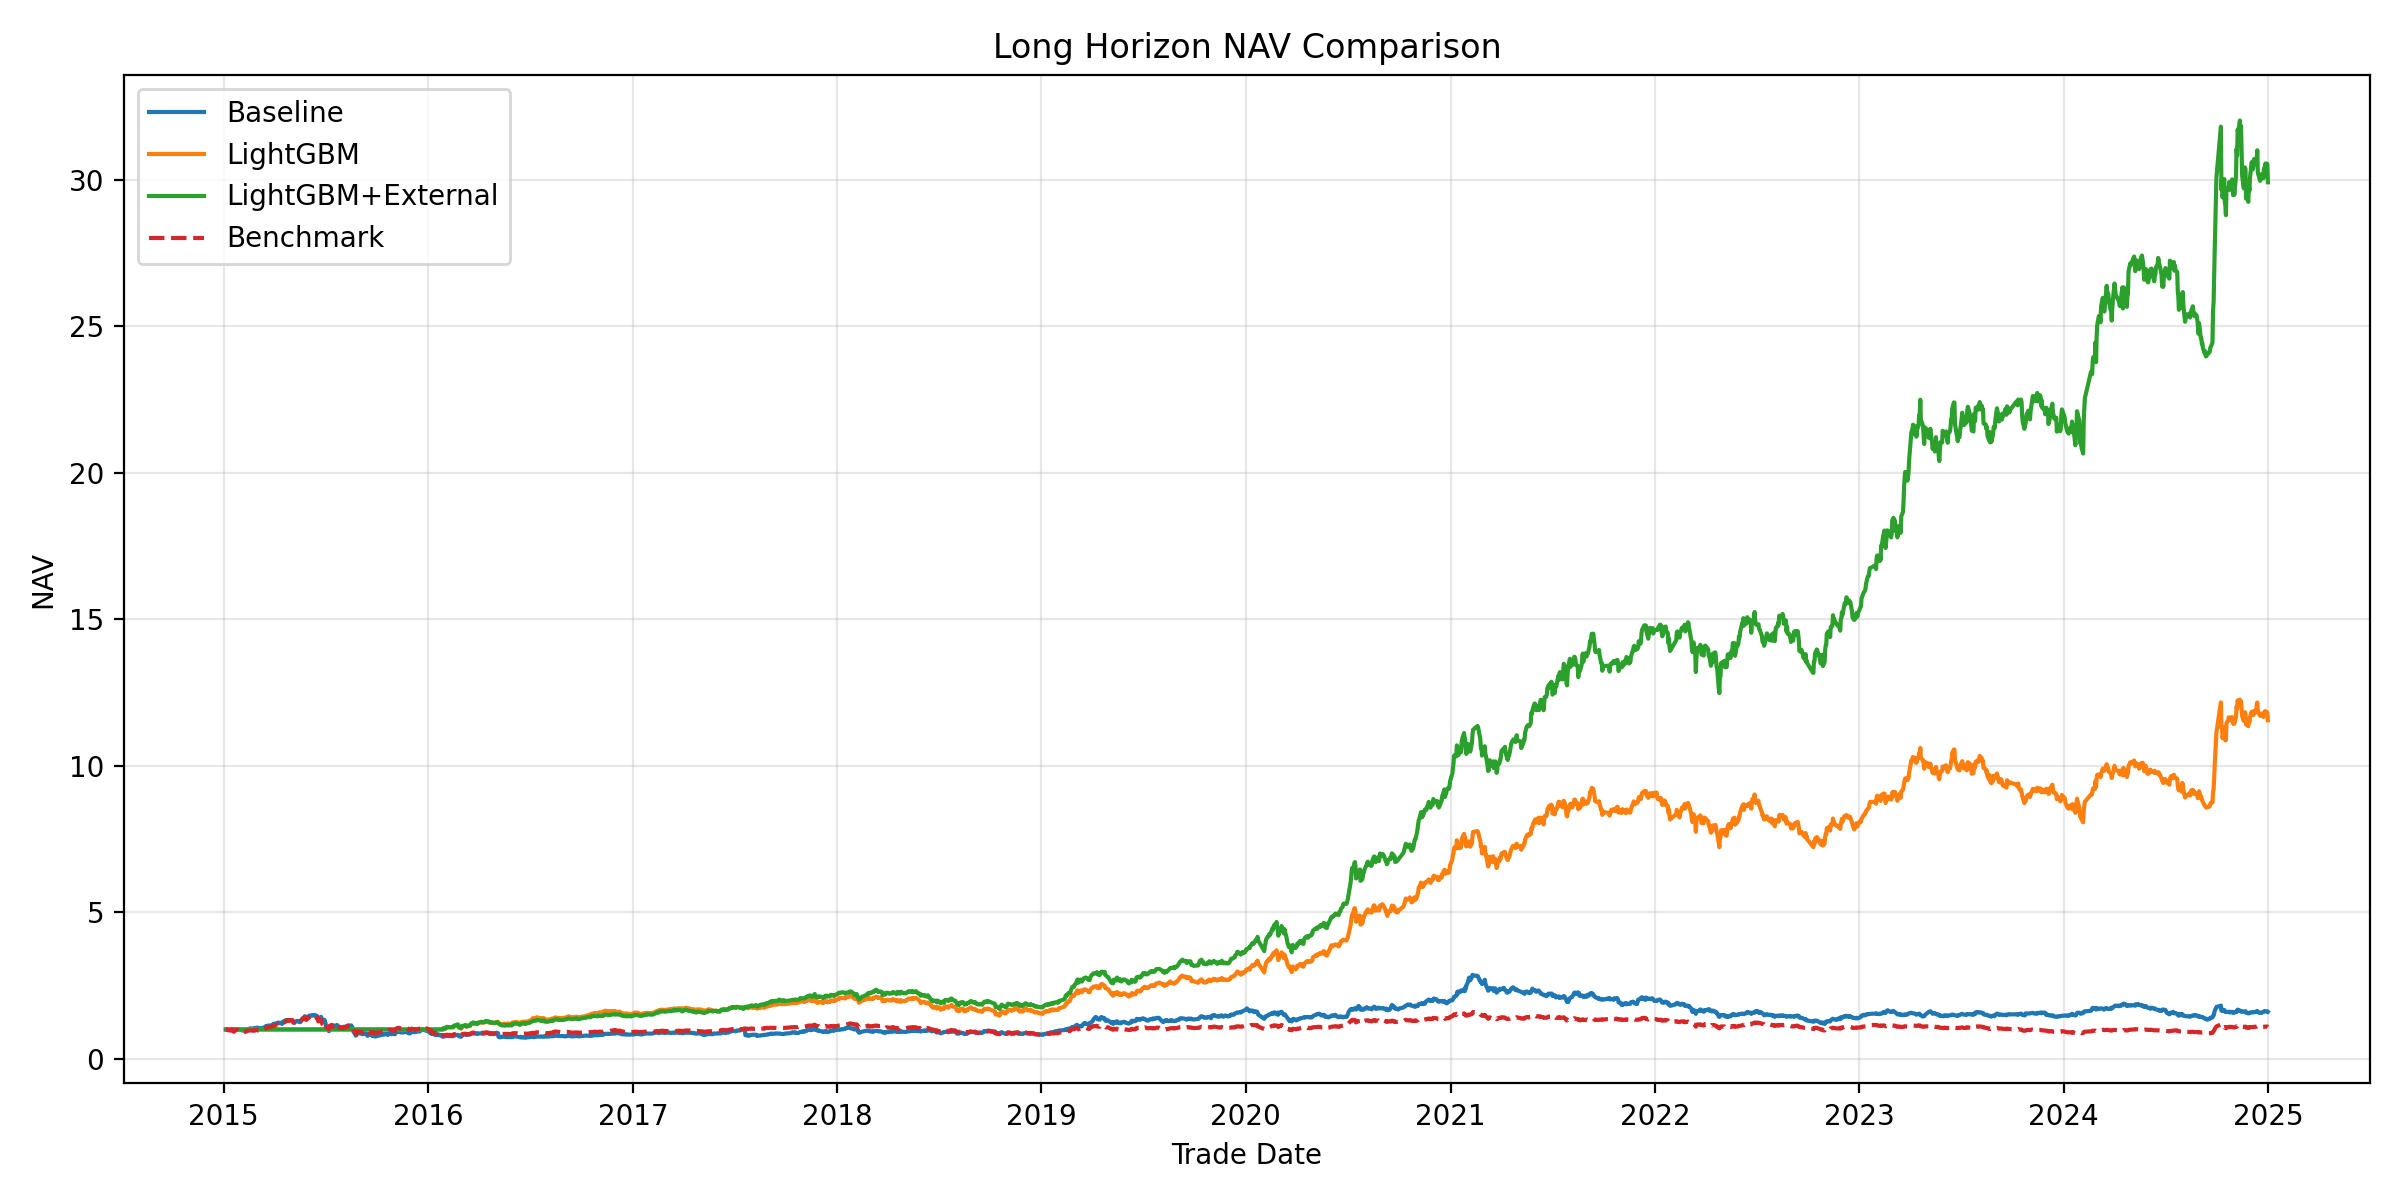
\includegraphics[width=0.85\textwidth]{figures/chart_01_long_horizon_nav.png}
\caption{长周期组合净值曲线对比（2015--2024）}
\label{fig:long_nav}
\end{figure}

\begin{figure}[htbp]
\centering
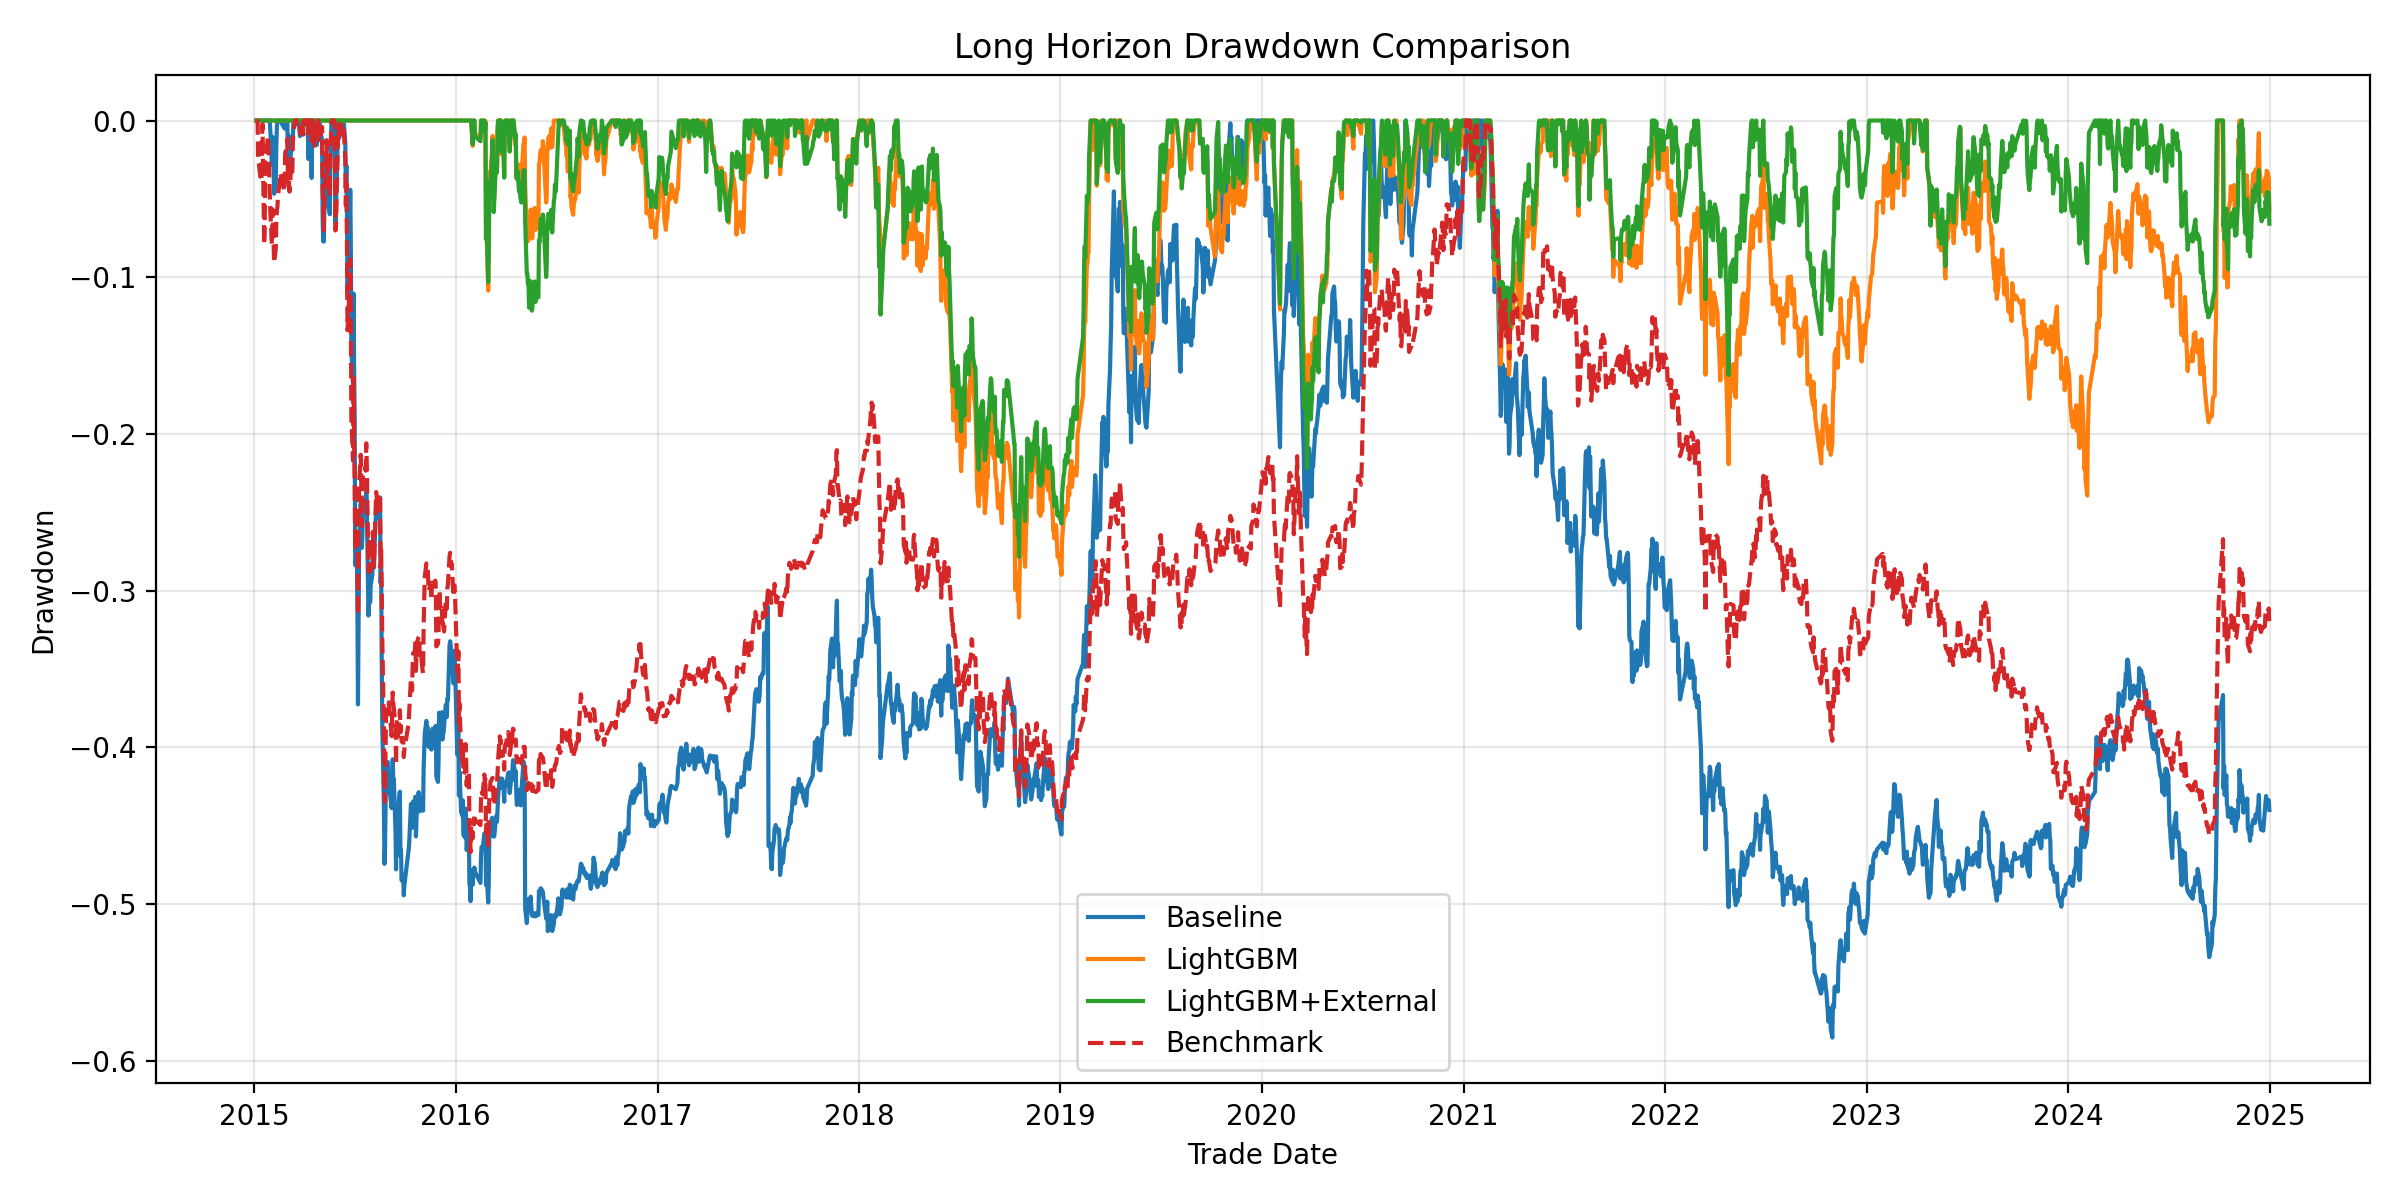
\includegraphics[width=0.85\textwidth]{figures/chart_03_long_horizon_drawdown.png}
\caption{长周期回撤曲线对比（2015--2024）}
\label{fig:long_dd}
\end{figure}

为理解增益来源，图~\ref{fig:feat_imp} 给出 LightGBM 滚动训练的特征重要性（按分裂次数）。可见质量与价值类基本面因子主导了模型决策：\texttt{grossprofitmargin}（$893$）、\texttt{ep\_ttm}（$874$）与 \texttt{bp}（$735$）位列前三；而宏观因子 \texttt{cn\_spread\_10y\_2y} 与 \texttt{m2\_yoy} 虽分裂次数中等，却具有最大的跨期方差（误差棒分别达 $\pm112$、$\pm105$），说明它们的使用强度高度依赖市场状态——这正是宏观因子作为 ``条件触发'' 变量、赋予模型动态风格轮动能力的体现。图~\ref{fig:regime} 进一步按市场状态分解绩效：在绝大多数牛熊区间，LightGBM 驱动与增强版本的 $IR$ 均显著高于基线，其中 $2019$--$2021$ 牛市 $IR$ 高达 $6.6$ 与 $9.3$；唯一的例外是 $2015$ 年杠杆牛市，机器学习策略出现明显负 $IR$（约 $-4.8$），原因在于该轮行情由非基本面的散户杠杆资金驱动，与模型所依赖的基本面信号背离。这一细致的状态依赖分析既肯定了算法在常态下的稳健增益，也诚实地揭示了其在极端非理性行情下的失效边界。

\begin{figure}[htbp]
\centering
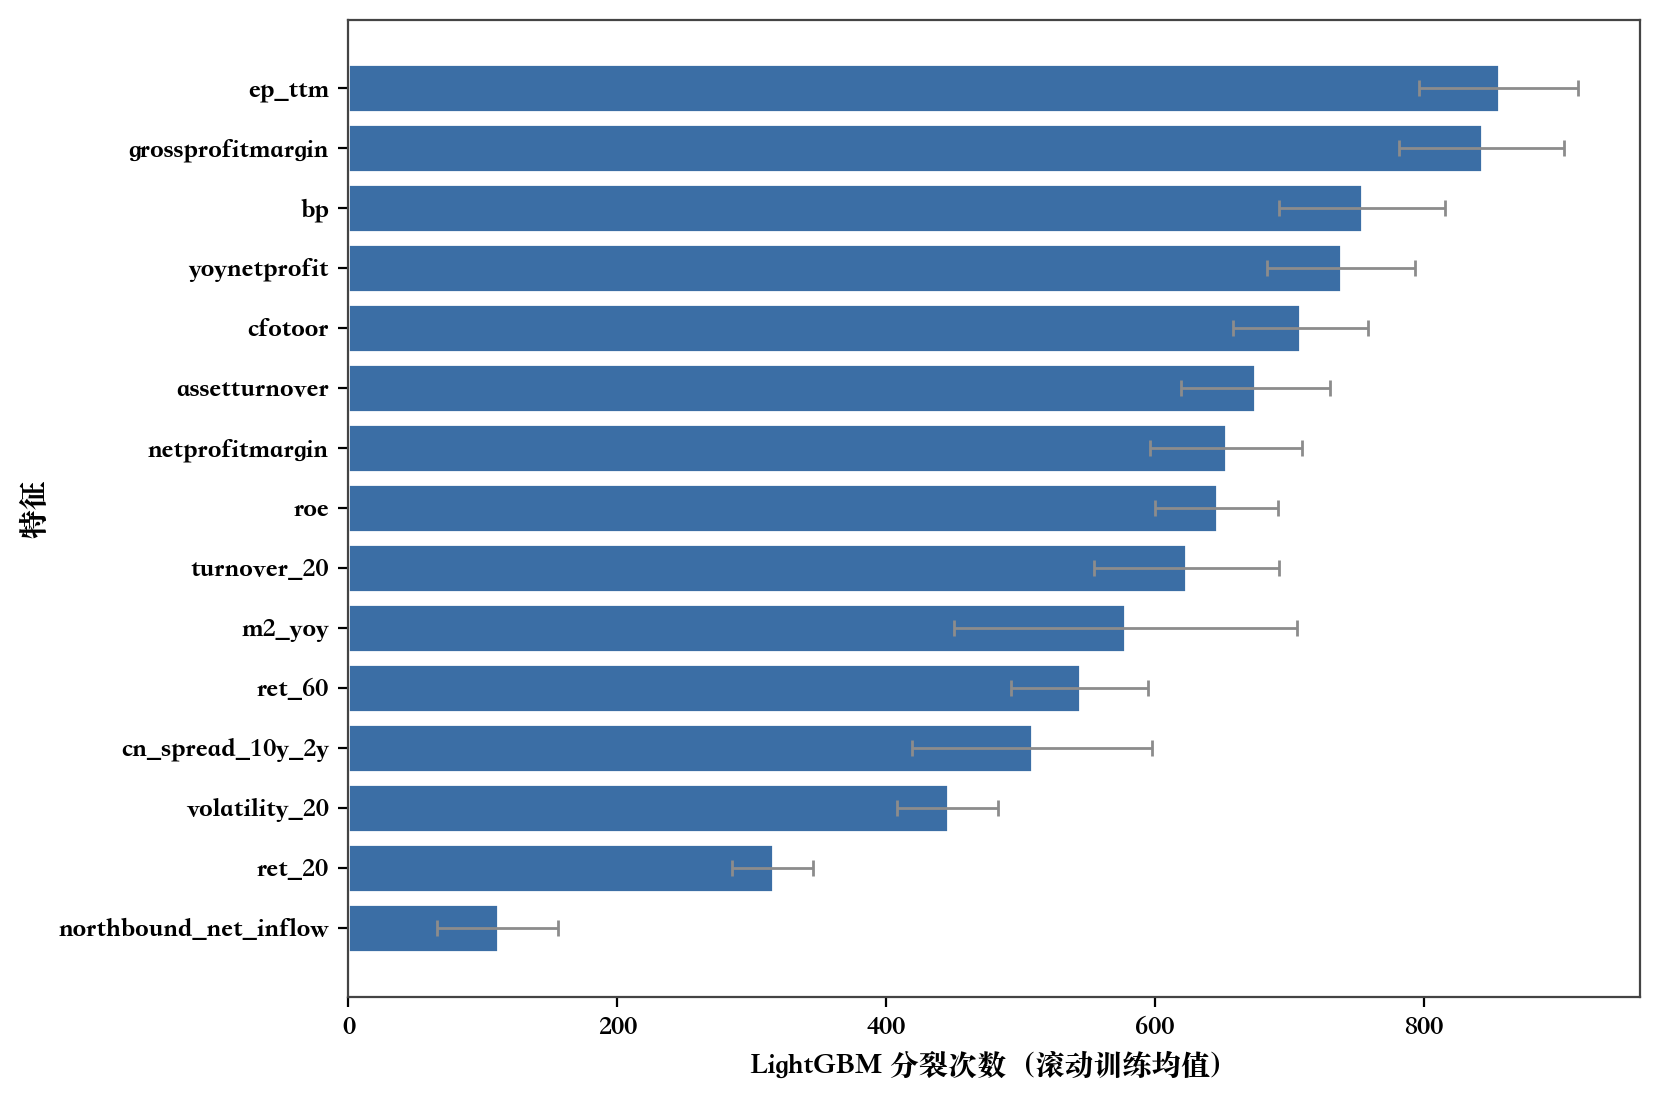
\includegraphics[width=0.85\textwidth]{figures/chart_07_feature_importance.png}
\caption{LightGBM 滚动训练的特征重要性（按分裂次数，误差棒为跨期标准差）}
\label{fig:feat_imp}
\end{figure}

\begin{figure}[htbp]
\centering
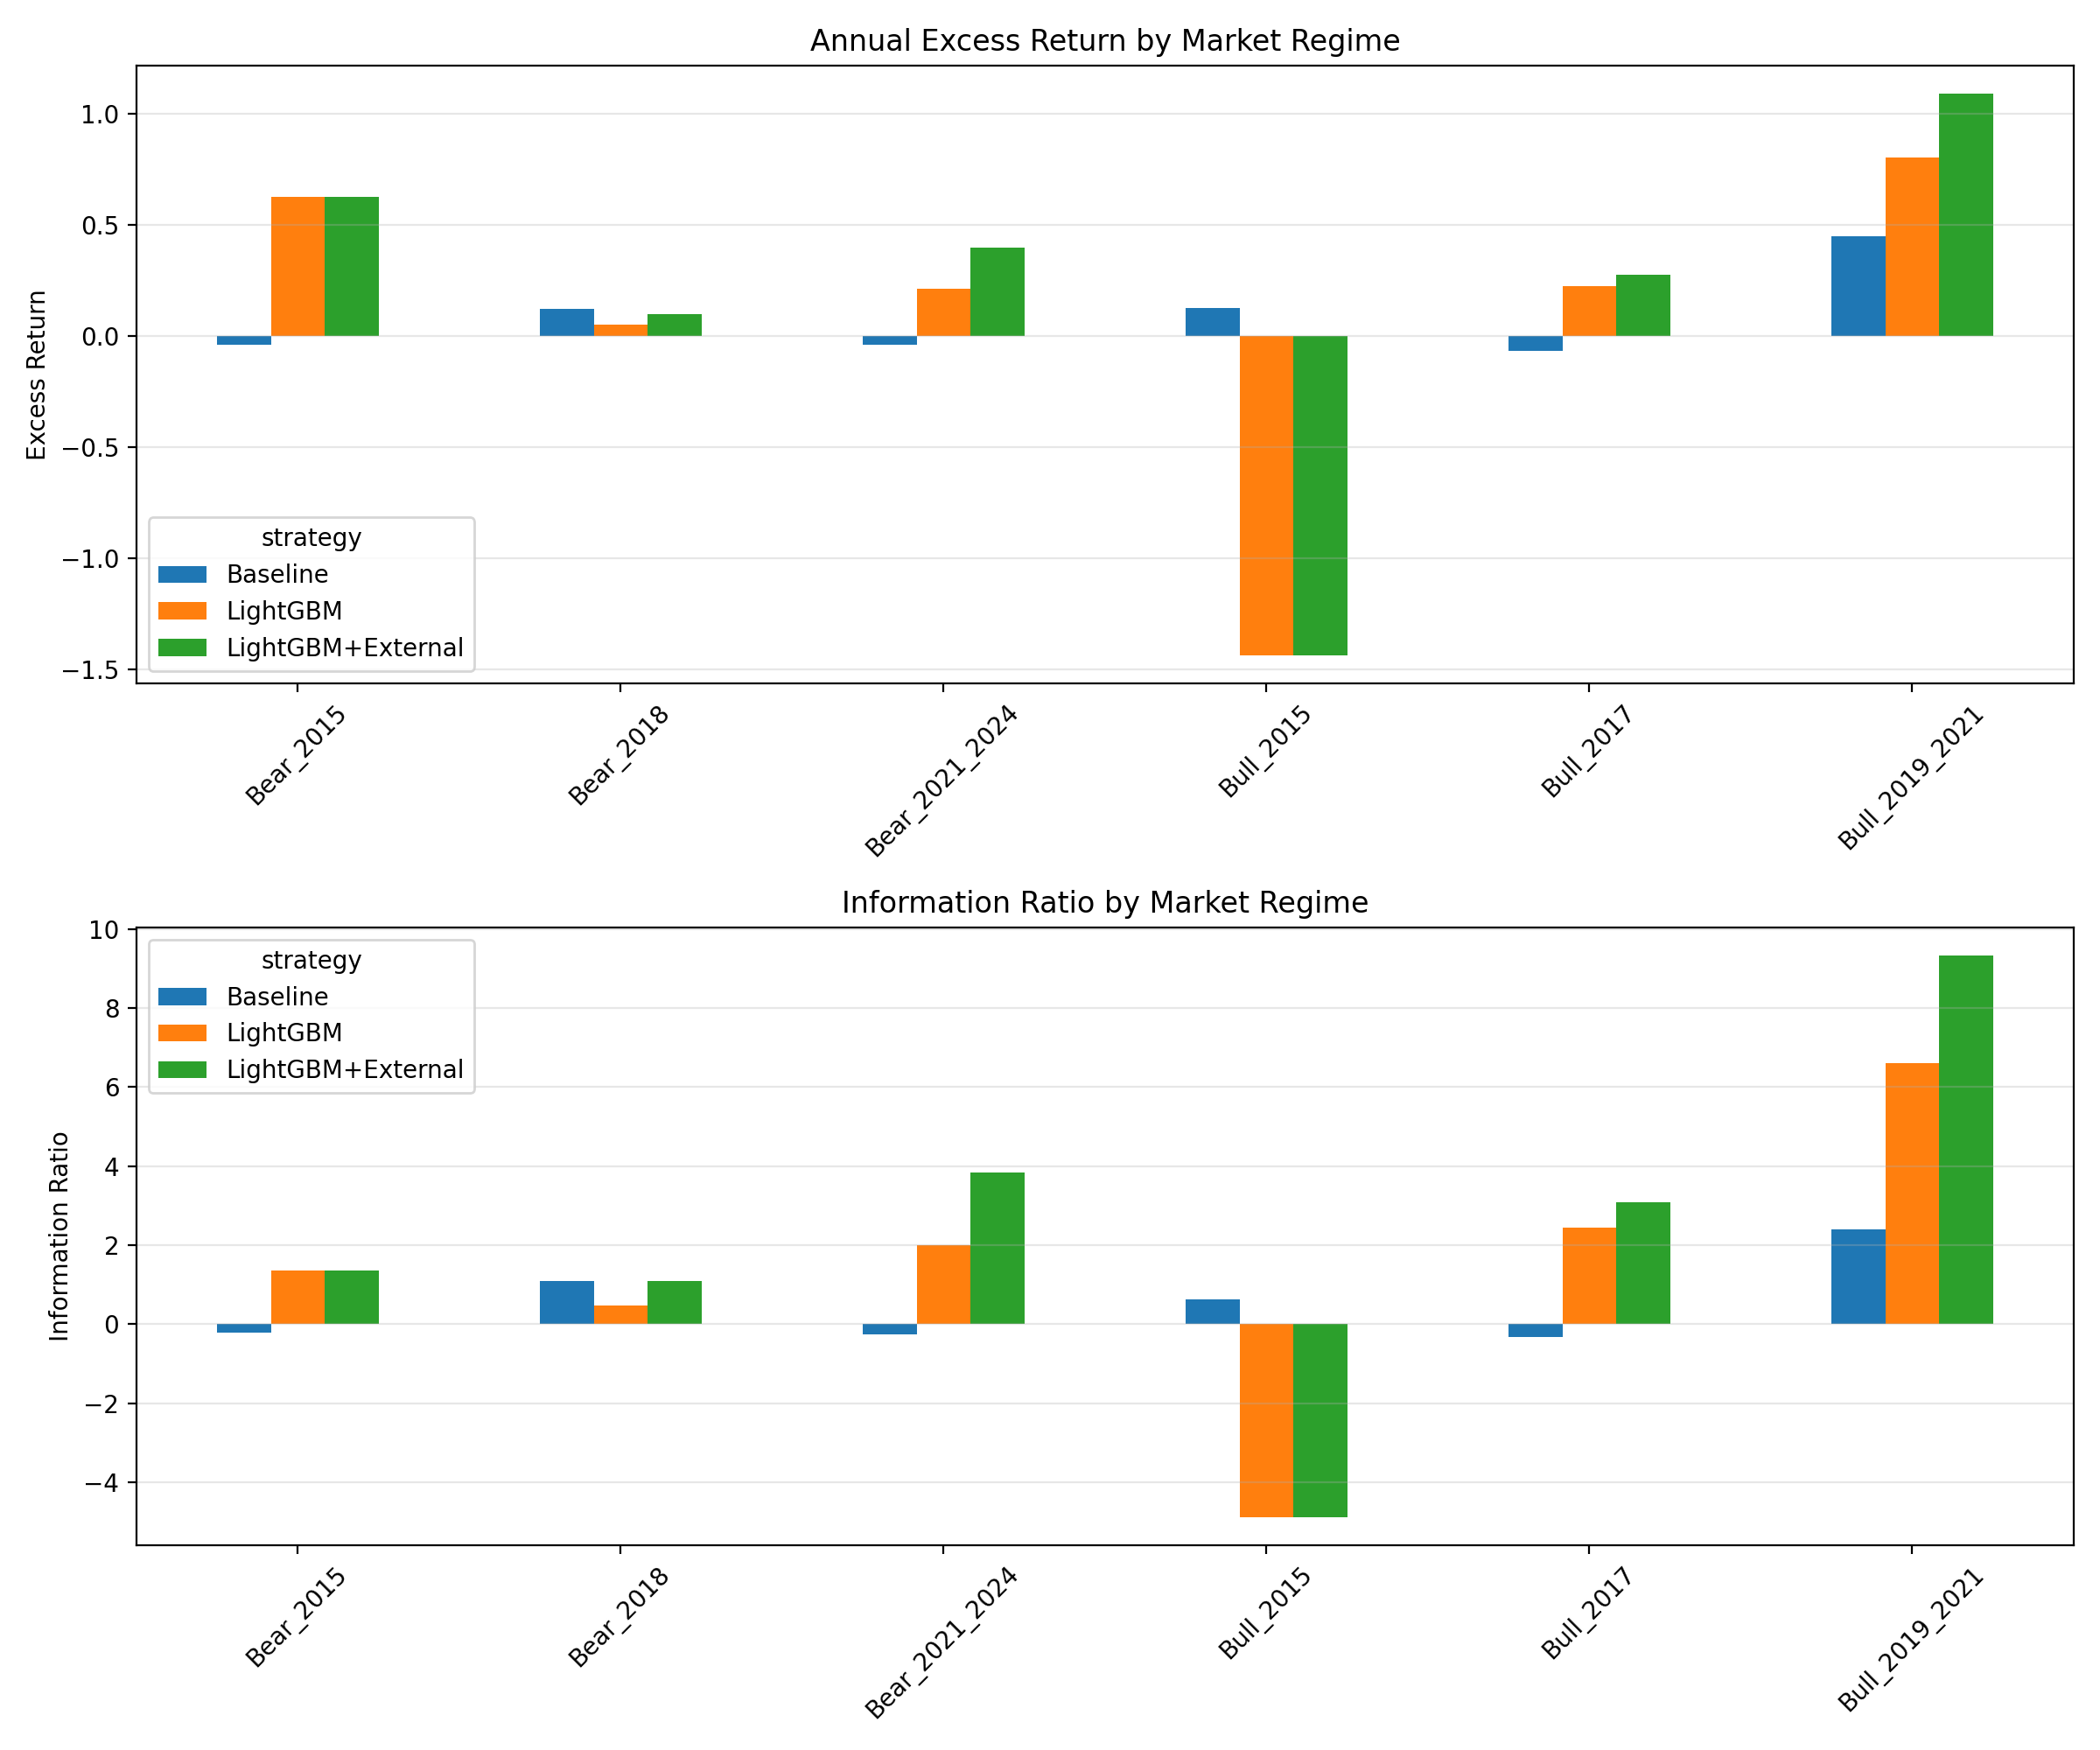
\includegraphics[width=0.85\textwidth]{figures/chart_08_regime_analysis.png}
\caption{按市场状态分解的年化超额收益与信息比率}
\label{fig:regime}
\end{figure}

\subsection{约束条件消融}
\label{subsec:ablation}
约束是压低 $TC$ 却保证可实施性的关键。表~\ref{tab:ablation} 逐一移除跟踪误差、行业偏离与换手率约束，考察其对绩效的影响。

\begin{table}[htbp]
\centering
\caption{约束条件消融（约束型 LightGBM，2015--2024）}
\label{tab:ablation}
\begin{tabular}{lccccc}
\toprule
\textbf{消融方案} & \textbf{年化超额} & \textbf{夏普} & \textbf{$IR$} & \textbf{最大回撤} & \textbf{年化换手} \\
\midrule
完整约束 & 28.07\% & 1.289 & 1.685 & -31.71\% & 2.08 \\
无跟踪误差约束 & 25.97\% & 1.141 & 1.472 & -33.62\% & 2.08 \\
无行业偏离约束 & 29.90\% & 1.394 & 1.760 & -32.47\% & 2.08 \\
无换手率约束 & 39.11\% & 1.791 & 2.334 & -29.83\% & 8.14 \\
\bottomrule
\end{tabular}
\end{table}

结果表明：移除跟踪误差约束反而使 $IR$ 下降（$1.685\!\to\!1.472$）并加深回撤，说明该约束在 A 股具有正向的风险控制价值；移除行业约束带来微弱的 $IR$ 提升（$1.685\!\to\!1.760$），代价是行业暴露失控；而移除换手率约束使 $IR$ 飙升至 $2.334$，但年化换手由 $2.08$ 暴涨至 $8.14$，落入脱离交易成本现实的 ``无摩擦乌托邦''。综合来看，完整约束版本是收益与可实施性之间的最优折衷，这与第二章传输系数理论的预期一致：合理的约束以可控的 $TC$ 损失换取了真实可交易性。

\subsection{不确定性感知扩展的评估}
\label{subsec:conformal}
本节评估第三章的不确定性感知扩展。表~\ref{tab:conformal} 在短周期样本上对比基线（不加权）与三种置信加权方案，图~\ref{fig:c3_metrics} 给出四项指标的可视化对照。

\begin{table}[htbp]
\centering
\caption{三种置信加权方案对照（2024--2025 约束型 LightGBM）}
\label{tab:conformal}
\begin{tabular}{lccccc}
\toprule
\textbf{方案} & \textbf{年化超额} & \textbf{夏普} & \textbf{$IR$} & \textbf{最大回撤} & \textbf{年化换手} \\
\midrule
基线（不加权） & 36.19\% & 2.413 & \textbf{2.893} & -9.22\% & 2.30 \\
alpha 缩放（$\beta{=}1$） & 24.47\% & 1.837 & 2.065 & -10.43\% & 2.30 \\
候选过滤（top $70\%$） & 30.49\% & 2.025 & 2.582 & -9.13\% & 2.61 \\
目标惩罚（$\gamma{=}0.1$） & 35.70\% & 2.420 & 2.821 & -9.50\% & 2.30 \\
\bottomrule
\end{tabular}
\end{table}

\begin{figure}[htbp]
\centering
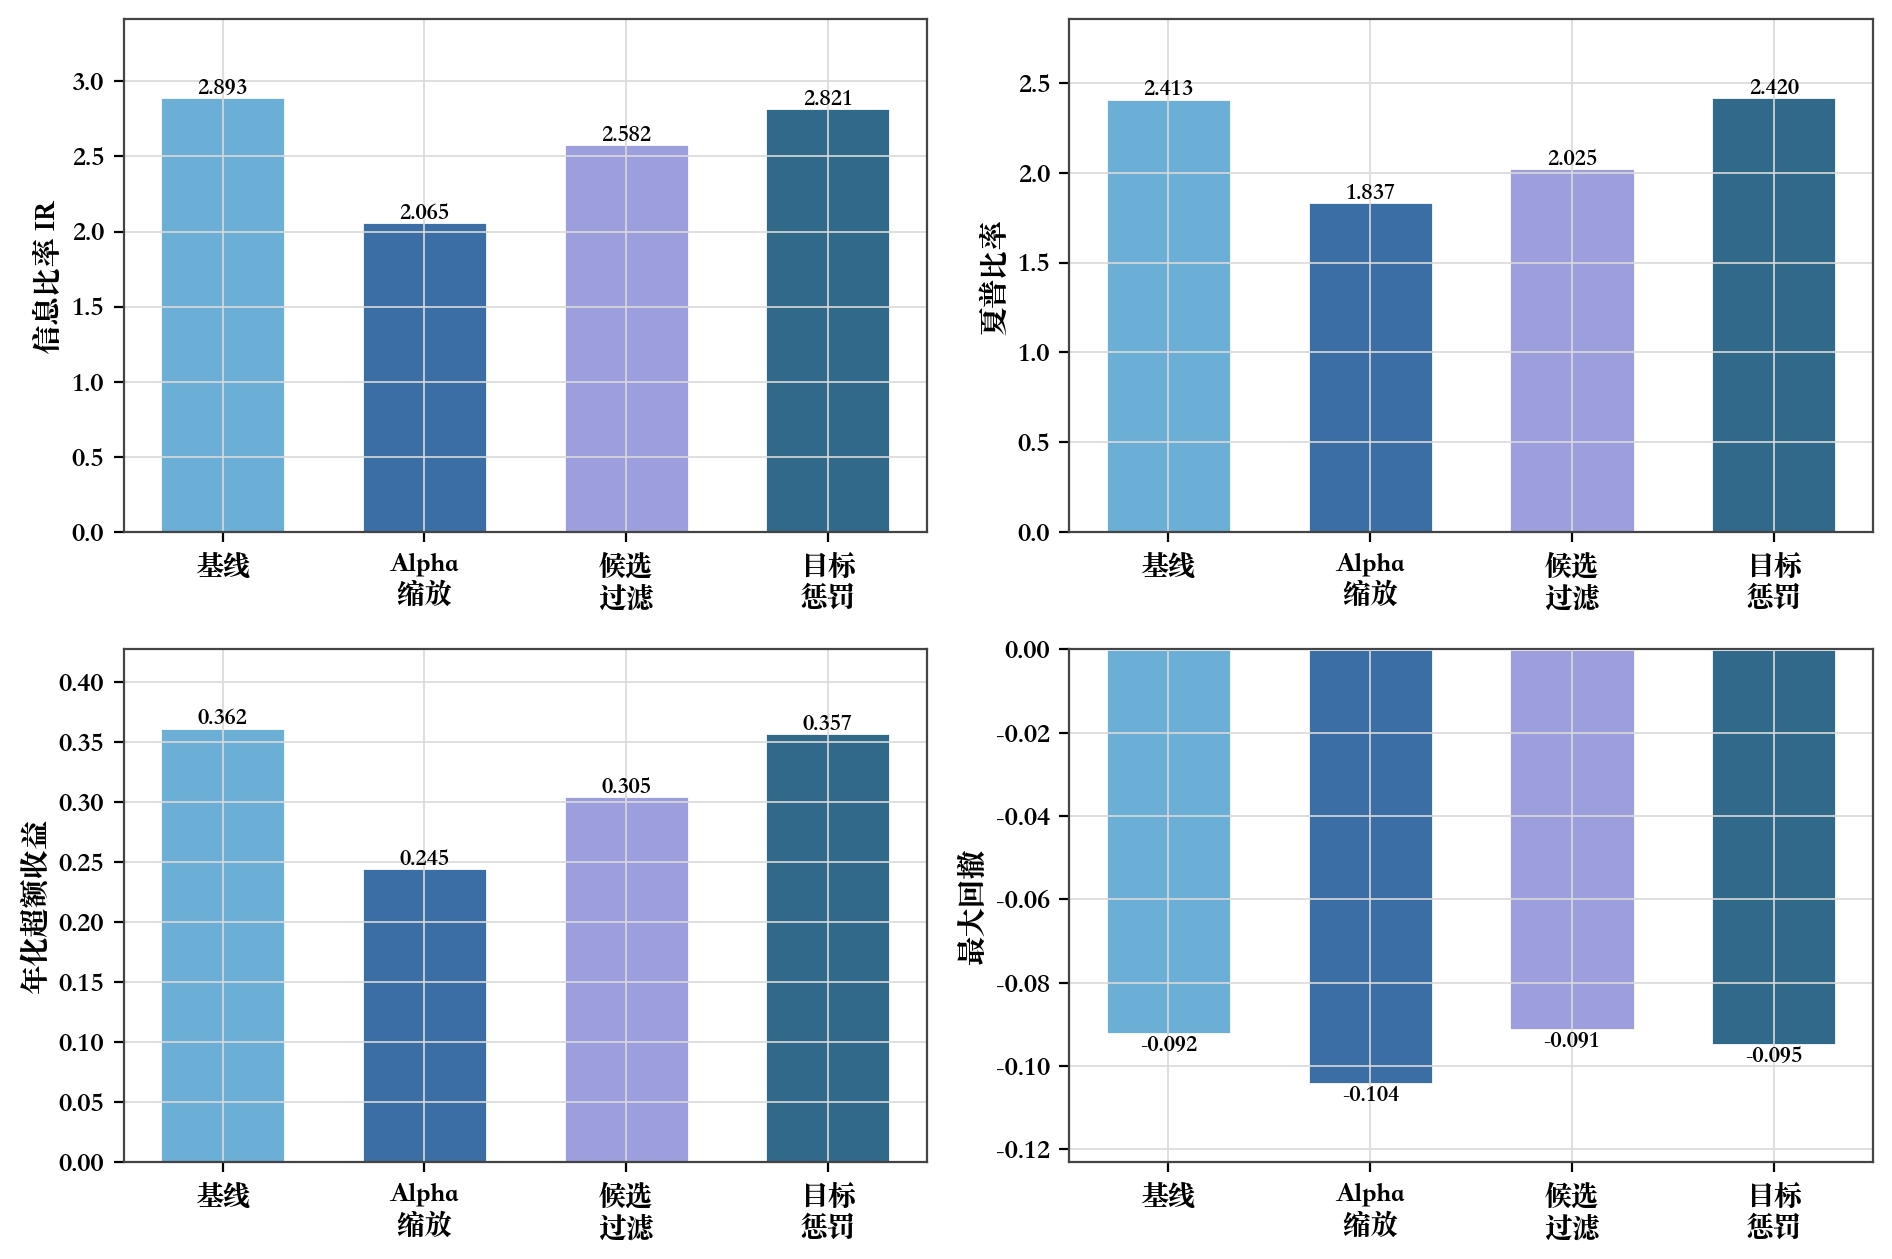
\includegraphics[width=0.95\textwidth]{figures/chart_c3_metrics_compare.png}
\caption{三种置信加权方案与基线的四项指标对照}
\label{fig:c3_metrics}
\end{figure}

一个出乎直觉但值得深究的结果是：\emph{三种置信加权方案的 $IR$ 均未超过不加权基线}（$2.893$）。由图~\ref{fig:c3_metrics} 可见，最激进的 alpha 缩放损失最大（$IR$ 降至 $2.065$，年化超额几乎腰斩），候选过滤居中（$2.582$），而最温和的目标惩罚最接近基线（$2.821$，夏普甚至以 $2.420$ 微超基线）。这一 ``越激进越受损'' 的单调关系提示：在 A 股环境下，Conformal 置信度信号本身可能存在系统性偏差，下文对其覆盖行为做进一步剖析。

\textbf{覆盖率与显著性水平敏感性。}图~\ref{fig:c3_alpha} 在 $2680$ 个真实预测点上扫描了三档显著性水平。左图显示，实测覆盖率（$86.6\%/80.9\%/70.8\%$）系统性地低于名义覆盖率（$95\%/90\%/80\%$）；右图显示，覆盖偏差稳定保持在 $-8.4\!\sim\!-9.2$ 个百分点，\emph{几乎不随显著性水平变化}。这说明该低覆盖并非区间过窄的偶发现象，而是可交换性假设在 A 股非平稳、强截面相关环境下被破坏所致的\emph{方法学层面的系统性偏差}。图~\ref{fig:c3_cov} 的月度覆盖轨迹进一步显示，覆盖率多数月份在 $0.81\!\sim\!0.91$ 波动，却在 $2024$ 年 $8$ 月骤降至 $0.43$——对应当月 A 股的剧烈波动，印证了分布漂移对覆盖的冲击。

\begin{figure}[htbp]
\centering
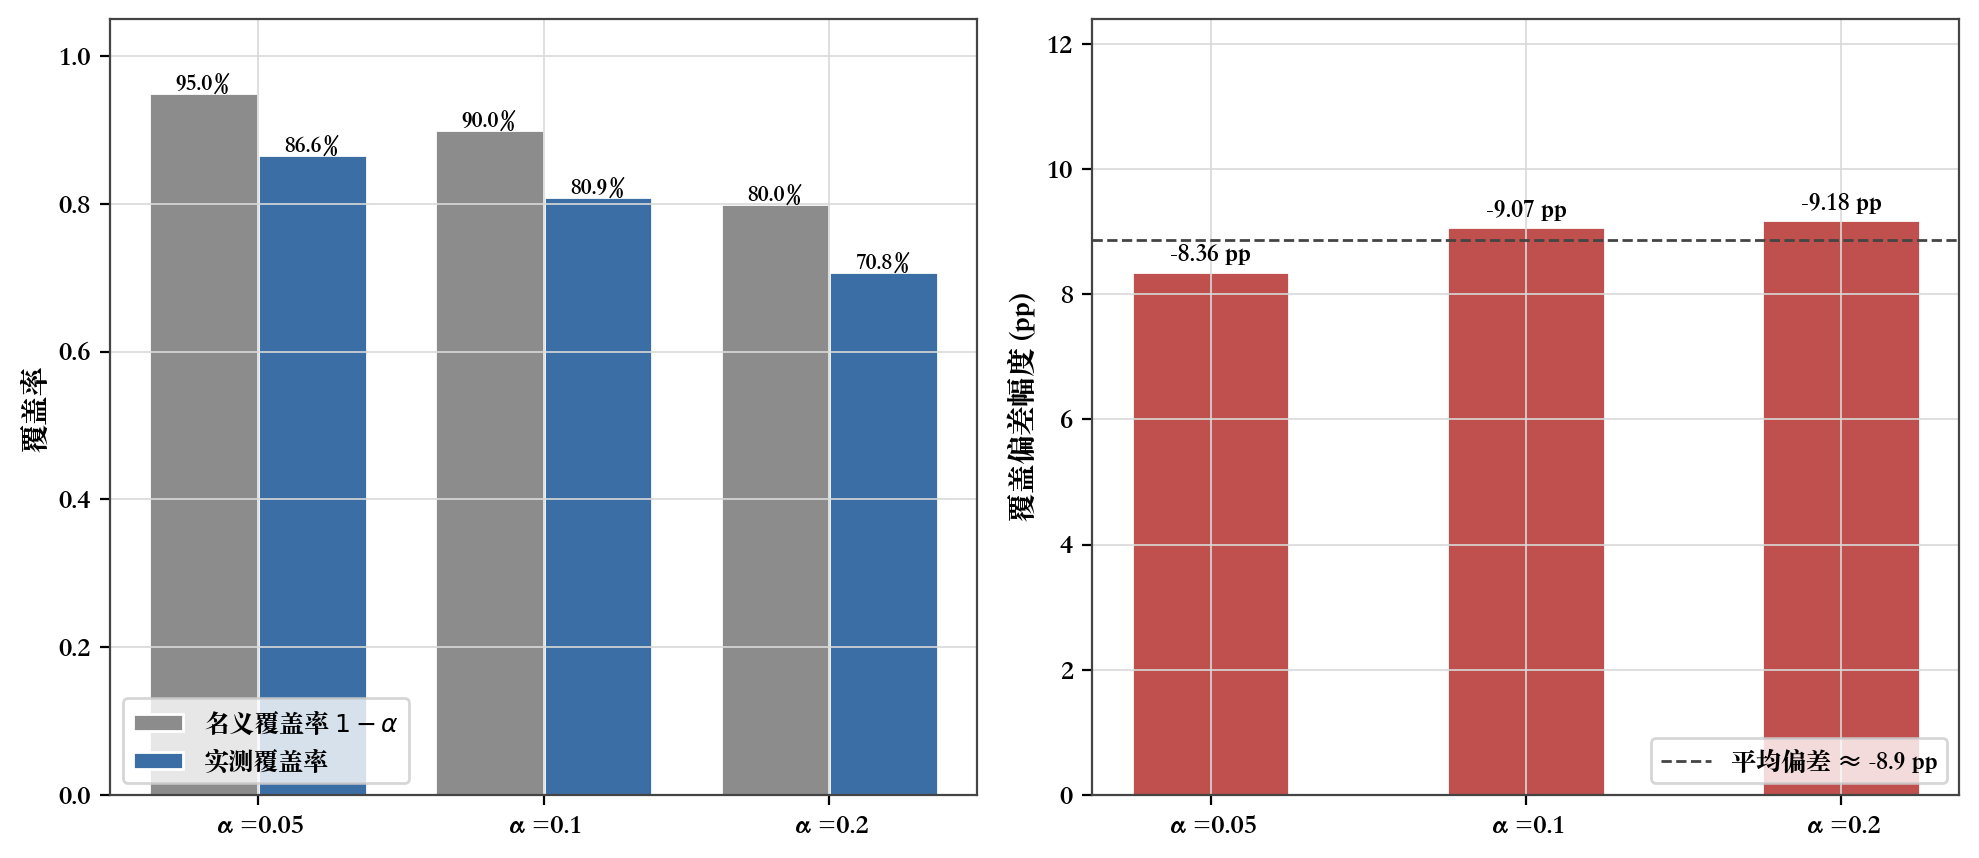
\includegraphics[width=0.95\textwidth]{figures/chart_c3_alpha_sensitivity.png}
\caption{Split Conformal 覆盖率对显著性水平的敏感性（偏差恒定约 $-9$ pp）}
\label{fig:c3_alpha}
\end{figure}

\begin{figure}[htbp]
\centering
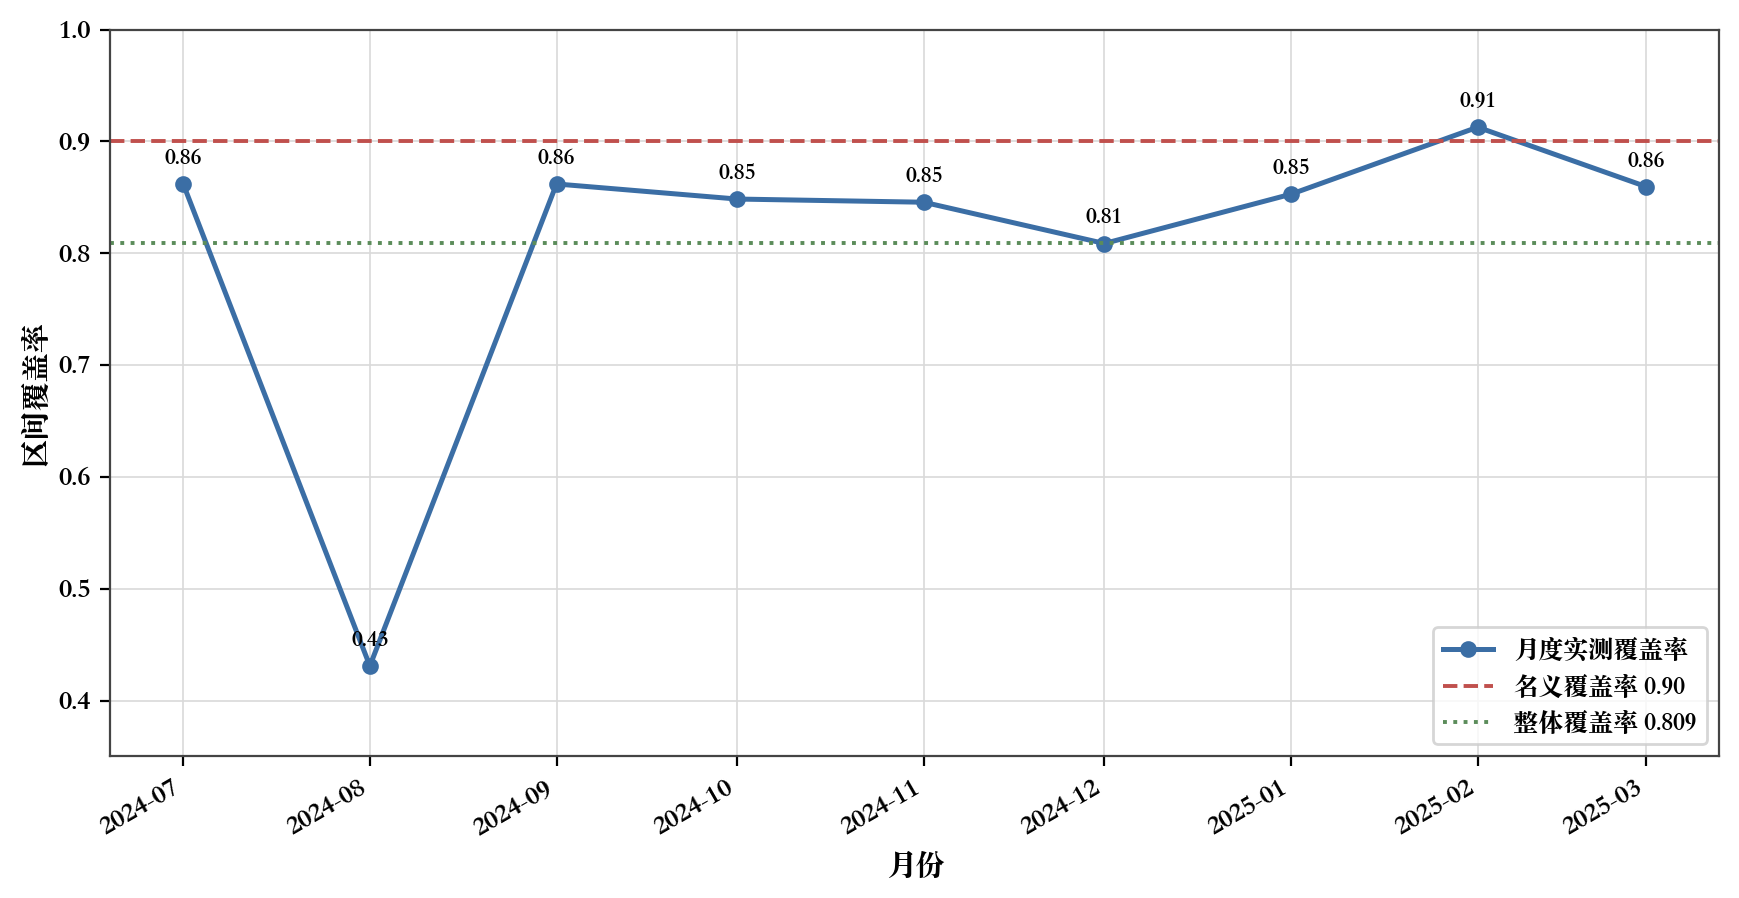
\includegraphics[width=0.85\textwidth]{figures/chart_c3_coverage_timeline.png}
\caption{Conformal 区间月度覆盖率与名义 $90\%$ 参考线}
\label{fig:c3_cov}
\end{figure}

\textbf{``高置信即过拟合'' 反向规律。}为揭示置信加权失效的机理，本文按置信度将预测分桶并统计各桶的 $IR$ 与命中率，结果如表~\ref{tab:buckets} 与图~\ref{fig:c3_bucket} 所示。

\begin{table}[htbp]
\centering
\caption{按 Conformal 置信度分桶的 $IR$ 与命中率（2024--2025）}
\label{tab:buckets}
\begin{tabular}{lccc}
\toprule
\textbf{分桶} & \textbf{样本数} & \textbf{$IR$} & \textbf{命中率} \\
\midrule
高置信（top $30\%$） & 804 & \emph{-0.140} & 0.425 \\
中置信（mid $40\%$） & 1072 & -0.028 & 0.419 \\
低置信（bottom $30\%$） & 804 & \textbf{+0.454} & 0.484 \\
\bottomrule
\end{tabular}
\end{table}

\begin{figure}[htbp]
\centering
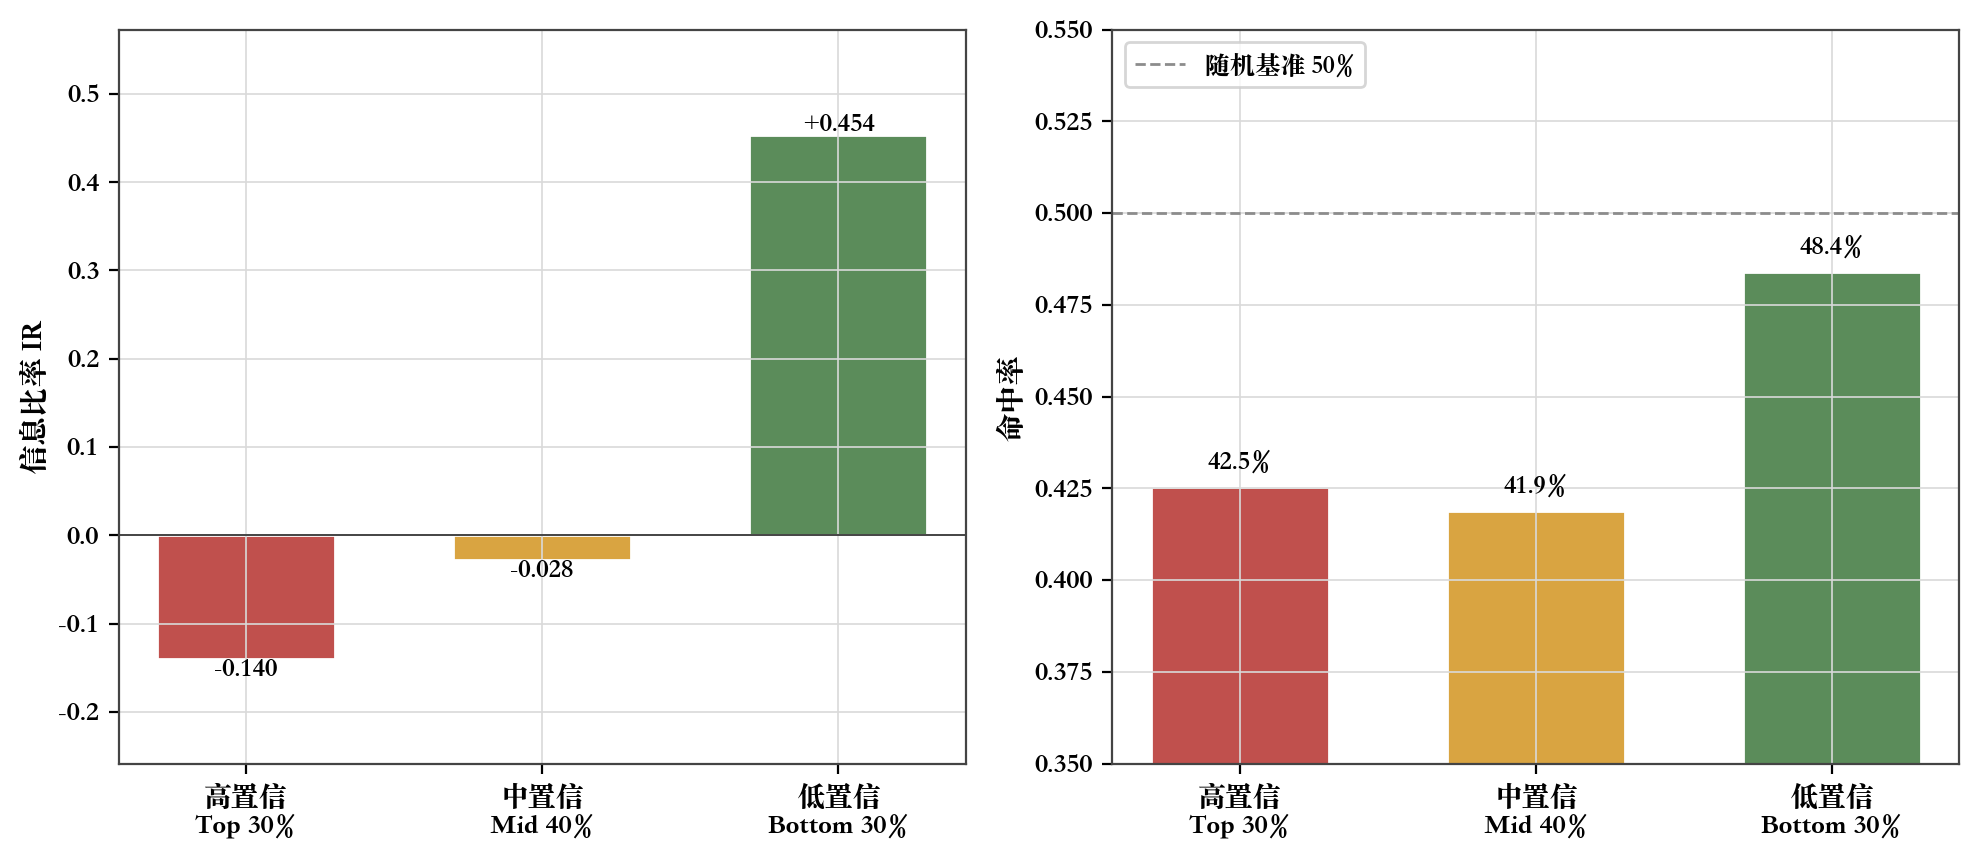
\includegraphics[width=0.95\textwidth]{figures/chart_c3_confidence_buckets.png}
\caption{按置信度分桶的 $IR$ 与命中率（高置信桶反而表现最差）}
\label{fig:c3_bucket}
\end{figure}

图~\ref{fig:c3_bucket} 左图清晰呈现一条\emph{反向单调}规律：高置信桶 $IR$ 为负（$-0.140$），随置信度下降，$IR$ 反而升至 $+0.454$；右图三桶命中率（$42.5\%/41.9\%/48.4\%$）则全部低于 $50\%$ 随机基准，且同样是低置信桶最高。这一 ``高置信即过拟合'' 的反向规律解释了表~\ref{tab:conformal} 的全部现象：由于 Conformal 的 ``高置信'' 在低信噪比 A 股中实际反映了\emph{残差分布的同质化（即过拟合程度）}而非\emph{预测可靠性}，因此越是激进地向高置信样本倾斜权重（alpha 缩放），损失越大；而仅做温和二次抑制的目标惩罚得以接近基线。本文进一步用 Mondrian 行业分组校准复测，发现真实数据上覆盖率仅由 $80.9\%$ 微升至 $81.3\%$、高置信桶 $IR$ 反而恶化至 $-0.205$，表明该反向规律相当稳健，仅靠行业分组无法矫正。

\textbf{自适应 CP 的矫正潜力。}上述系统性低覆盖指向了改进方向。本文以 Gibbs 与 Cand\`es\cite{Gibbs2021ACI} 的 ACI 更新规则 $\alpha_{t+1}=\alpha_t+\eta\,(\mathbb{1}[y_t\notin C_t]-\alpha_{\text{target}})$ 在 $3276$ 个日度预测点上做简化模拟，结果如表~\ref{tab:aci} 所示：在低学习率 $\eta\in[0.005,0.01]$ 下，估算覆盖率回升至 $89.5\%$--$89.7\%$，相比静态 Split CP 的 $80.9\%$ \textbf{矫正了约 $80\%$ 的覆盖偏差}；学习率过大（$\eta=0.1$）则因 $\alpha_t$ 自身震荡而恶化覆盖。该结果定性地验证了自适应 CP 在 A 股矫正覆盖偏差的可行性，其正式实现与端到端集成留作未来工作。

\begin{table}[htbp]
\centering
\caption{Adaptive Conformal Inference 简化模拟：学习率 $\eta$ 对覆盖率的影响}
\label{tab:aci}
\begin{tabular}{cccc}
\toprule
$\eta$ & \textbf{平均 $\alpha_t$} & \textbf{最终 $\alpha_t$} & \textbf{估算覆盖率} \\
\midrule
0.005 & 0.103 & 0.104 & \textbf{89.7\%} \\
0.010 & 0.105 & 0.108 & \textbf{89.5\%} \\
0.050 & 0.126 & 0.139 & 87.4\% \\
0.100 & 0.152 & 0.178 & 84.8\% \\
\midrule
\multicolumn{4}{l}{\emph{对照：静态 Split CP 实测覆盖率 $= 80.9\%$（名义 $90\%$）}} \\
\bottomrule
\end{tabular}
\end{table}

\subsection{综合策略对比与稳健性}
\label{subsec:robustness}
表~\ref{tab:final} 在同一短周期面板上横向对比三种代表性策略：等权基线、LightGBM 加约束优化器、以及叠加 Conformal 目标惩罚的优化器。

\begin{table}[htbp]
\centering
\caption{三策略综合对比（2024--2025 真实数据）}
\label{tab:final}
\begin{tabular}{lccccc}
\toprule
\textbf{策略} & \textbf{年化超额} & \textbf{Sharpe} & \textbf{$IR$} & \textbf{最大回撤} & \textbf{年化换手} \\
\midrule
等权基线（无优化器） & 7.43\% & 0.852 & 0.732 & -12.85\% & 5.13 \\
LightGBM $+$ 约束优化器 & 66.31\% & 3.336 & \textbf{5.839} & \textbf{-9.22\%} & \textbf{2.30} \\
$+$ Conformal 目标惩罚 & 65.41\% & 3.342 & 5.634 & -9.50\% & 2.30 \\
\bottomrule
\end{tabular}
\end{table}

对比可见：相对等权基线（$IR\ 0.732$、换手 $5.13$），约束优化器在将 $IR$ 提升至 $5.839$ 的同时，把换手压到 $2.30$、回撤收窄至 $-9.22\%$，再次印证算法~\ref{alg:cpo} 在收益与可实施性上的双重价值。Conformal 目标惩罚版本 $IR$ 略低（$5.634$），与第~\ref{subsec:conformal} 节的结论一致——在短样本低信噪比下，置信加权尚不能带来正贡献，但其温和形式未显著损害绩效，且为不确定性感知优化保留了可扩展的接口。

\textbf{持仓数与传输系数。}本文扫描了不同持仓数下 LightGBM 等权策略（不启用优化器）的 $IR$：Top $10/20/30/50$ 分别为 $8.26/7.13/6.37/4.98$，呈单调递减——持仓越集中，alpha 越被放大。Top $20$ 的等权上限 $IR\ 7.13$ 与表~\ref{tab:final} 中加优化器后的 $IR\ 5.839$ 对照，恰好量化了传输系数 $TC\approx 5.839/7.13\approx 0.82$，即优化器在严格风控下仍传输了约 $82\%$ 的理论 alpha，与第二章 $IR=TC\cdot IC\cdot\sqrt{N}$ 的理论框架定量吻合。

\textbf{严格样本外验证。}为检验可投资性，本文冻结训练好的模型、禁止滚动重训，在 $2025$ 年做严格样本外回测，结果如表~\ref{tab:oos} 与图~\ref{fig:oos2024}--\ref{fig:oos2015} 所示。以近期一年（2024）训练时，LightGBM 仍稳定击败基线（$+$外部 $IR\ 2.857$ vs 基线 $1.460$）；但当训练窗口扩展到 $2015$--$2024$ 全历史时，模型反而出现负 $IR$（$-0.283$）。图~\ref{fig:oos2024} 显示近期训练下增强组合（绿）与 LightGBM（橙）净值显著高于基准；而图~\ref{fig:oos2015} 则呈现相反图景——长历史训练的两条机器学习曲线（橙、绿）反被基线（蓝）超越。这一对照鲜明地揭示了 A 股的强非平稳性：过时的历史风格会成为噪声，故近期短窗口滚动重训才是可投资性的关键，这也为第三章的月度重训设计提供了实证支撑。

\begin{table}[htbp]
\centering
\caption{严格样本外验证（信息比率，$\to$ 2025 测试）}
\label{tab:oos}
\begin{tabular}{lccc}
\toprule
\textbf{训练设定} & \textbf{基线} & \textbf{Factor-only} & \textbf{$+$External} \\
\midrule
2024 $\to$ 2025（近期窗口） & 1.460 & 2.729 & \textbf{2.857} \\
2015--2024 $\to$ 2025（长历史） & 1.460 & \emph{-0.482} & \emph{-0.283} \\
\bottomrule
\end{tabular}
\end{table}

\begin{figure}[htbp]
\centering
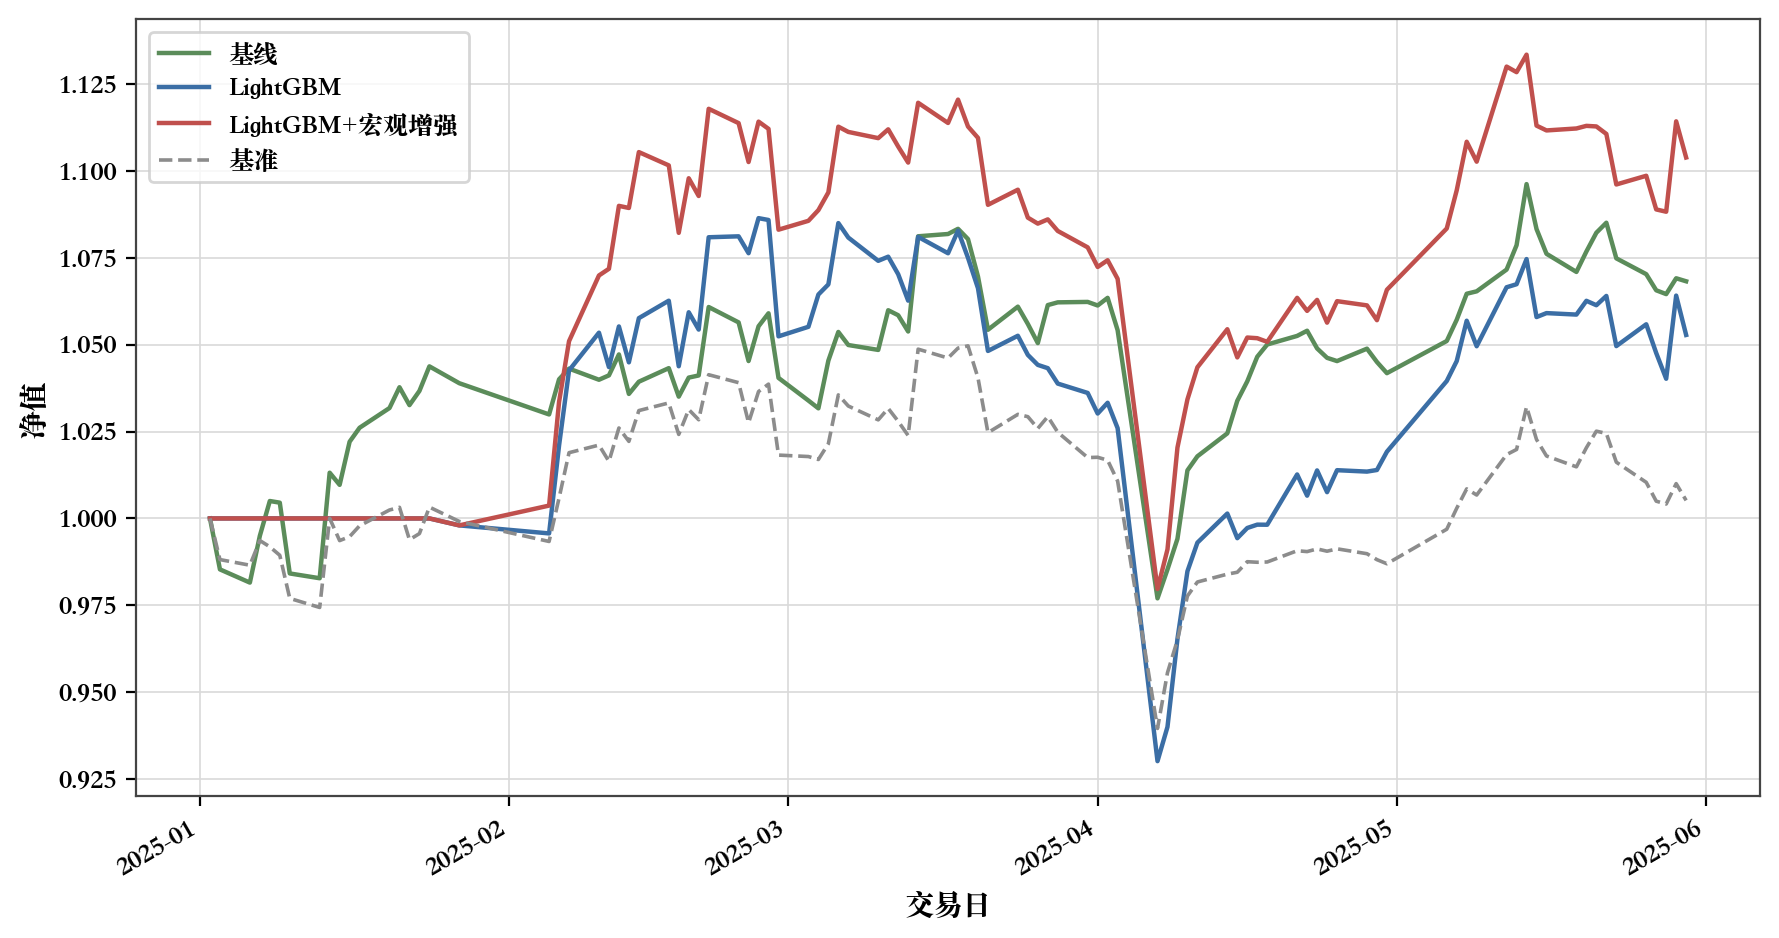
\includegraphics[width=0.8\textwidth]{figures/chart_04_strict_oos_2025_nav_2024train.png}
\caption{严格样本外：近期（2024）训练 $\to$ 2025 测试净值}
\label{fig:oos2024}
\end{figure}

\begin{figure}[htbp]
\centering
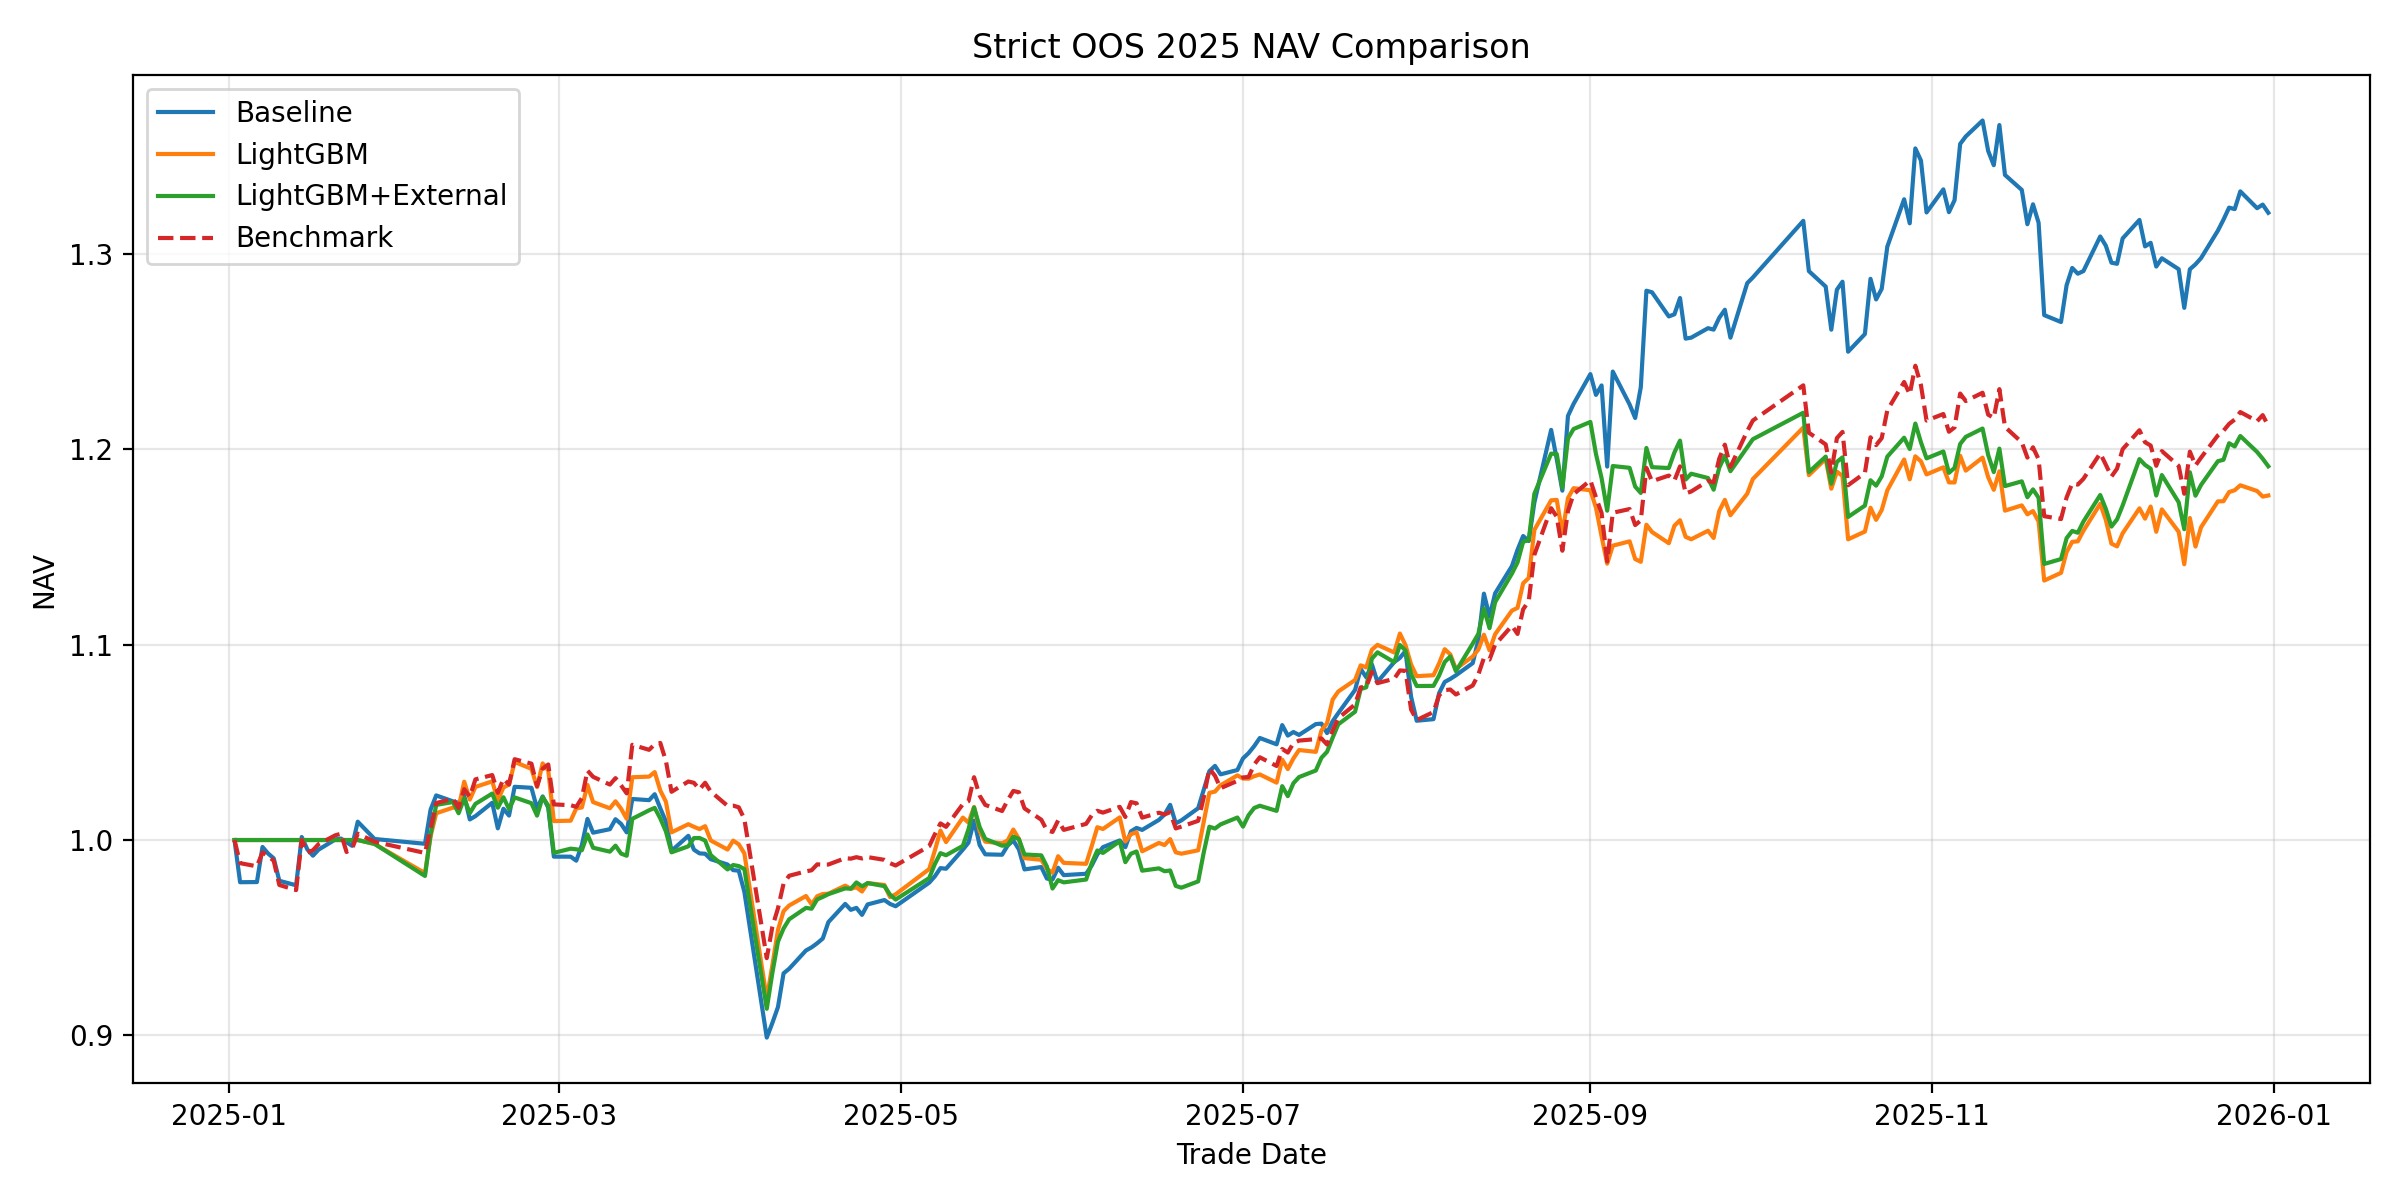
\includegraphics[width=0.8\textwidth]{figures/chart_05_strict_oos_2025_nav_2015train.png}
\caption{严格样本外：长历史（2015--2024）训练 $\to$ 2025 测试净值}
\label{fig:oos2015}
\end{figure}

\textbf{随机种子稳定性。}为排除结果依赖于幸运种子，本文以 $5$ 个不同随机种子重跑 LightGBM 等权 Top20，$IR$ 均值 $7.01$、标准差 $0.13$，变异系数仅 $1.85\%$，远低于一般认为可疑的 $5\%$--$10\%$ 阈值，表明所报告的绩效是稳健结果而非挑选所得。

\section{本章小结}
\label{sec:exp_summary}
本章以与基线的对比论证了第三章算法的有效性。约束组合优化算法在长周期上将 $IR$ 由 $0.237$ 提升至 $2.449$、最大回撤由 $-58.53\%$ 收敛至 $-25.37\%$，约束消融、传输系数 $TC\approx0.82$ 与严格样本外验证从多个角度证实了其稳健性与可实施性。对不确定性感知扩展的系统评估则表明：在 A 股低信噪比环境下，Conformal 置信度存在约 $9$ 个百分点、与显著性水平无关的系统性低覆盖，并伴随 ``高置信即过拟合'' 的反向规律，致使置信加权暂未带来正向收益；而简化的 ACI 模拟可矫正约 $80\%$ 的覆盖偏差，为后续改进指明了方向。

\chapter{总结与展望}

\section{工作总结}
本文以沪深 300 指数增强为应用场景，围绕其核心量化算法——带约束的组合优化——展开了优化设计与实现。主要工作与结论如下。

第一，本文从主动管理基本定律 $IR=TC\cdot IC\cdot\sqrt{N}$ 出发，明确了组合优化（最大化传输系数 $TC$）在指数增强策略中的核心地位，并将其在 A 股的落地难题归结为协方差病态与低信噪比预测不确定性两重挑战。

第二，针对协方差病态，本文设计并实现了约束型多因子组合优化算法：以 Ledoit-Wolf 缩减与最小特征值修正应对 ``误差最大化''，以带跟踪误差、行业、权重与换手约束的二次规划保证可实施性，并以 OSQP$\to$CLARABEL$\to$SCS 三级回退保证数值鲁棒性。长周期实证表明，该算法将信息比率由静态多因子的 $0.237$ 提升至 $2.449$，最大回撤由 $-58.53\%$ 收敛至 $-25.37\%$，并以约 $0.82$ 的传输系数高效兑现了理论 alpha。

第三，针对预测不确定性，本文将 Split 与 Mondrian Conformal Prediction 引入组合优化，设计了 alpha 缩放、候选过滤与目标惩罚三种置信加权方案。对其行为的系统评估不仅给出了完整的工程实现，更揭示出 A 股环境下 Conformal 置信度约 $9$ 个百分点、与显著性水平无关的系统性低覆盖，以及 ``高置信即过拟合'' 的反向规律；简化的自适应 CP 模拟进一步表明，该覆盖偏差中约 $80\%$ 可被在线学习率矫正。这一发现既是对置信加权失效机理的深入解释，也为不确定性感知组合优化在低信噪比市场的改进提供了明确依据。

\section{局限与未来展望}
\label{sec:future_work}
本文工作仍受样本规模与方法选择的制约，结合实验结论，未来可在以下方向继续深入。

\textbf{自适应 Conformal Prediction 的端到端集成。}第~\ref{subsec:conformal} 节揭示的系统性低覆盖与反向规律，根源在于静态 Split CP 对可交换性的依赖。未来可将 Temporal CP\cite{Aydin2025TCP}、变点感知 CP\cite{Sun2025CPTC} 或免训练的 ResCP\cite{Neglia2026ResCP} 正式实现并端到端接入优化器，以在线方式矫正第~\ref{subsec:conformal} 节量化的 $-9$ 个百分点偏差，进而检验置信加权能否在矫正覆盖后转为正贡献。

\textbf{协方差估计的升级。}本文的 Ledoit-Wolf 缩减是线性收缩，未来可引入生成式方法（如扩散因子模型）所产出的多场景合成收益来估计协方差，以更灵活地刻画 A 股的非线性相关结构，替代或补充式~\eqref{eq:te} 中的 $\Sigma$。

\textbf{分布鲁棒的组合优化。}本文以惩罚或缩放的方式 ``软性'' 利用不确定性，未来可探索分布鲁棒优化（DRO），将预测不确定性直接写入约束的 ``最坏情形'' 形式，使可行域本身具备对预测误差的免疫力，与本文的置信加权形成互补。

\textbf{更长样本与跨市场验证。}受 A 股强非平稳性影响，短周期结论需谨慎外推。未来将在更长样本与其他宽基指数（如中证 500、中证 1000）上复测算法的稳健性，并系统评估交易成本模型对传输系数的影响。
